% Template KLTN cho SV trường ĐHKHTN
% Liên hệ: bhthong@fit.hcmus.edu.vn
% Last update: 

% Chú ý: đọc các phần chú ý đóng khung của file này và chỉnh lại cho phù hợp.
% Trước khi build, xóa hết các file được tạo ra trong quá trình build trước đó, và build theo thứ tự: BIB > PDF > PDF.
% Nếu cập nhật tài liệu tham khảo, cũng cần build lại theo cách trên.

% Muc tieu la viet Paper
% 1. Introduction
%      Motivation / Problem statement
%      Relative works
%      Scope & Research objectives
%      Thesis Contribution
% 2. {Kien thuc can biet de doc luan} / Fundamental basis
%      Definition
%      ...
%      definition LLM
%      definition finetune
%      definition RAG
% 3. Proposed approach
%      {Kien truc he thong}
%      {Tung component cua he thong}
% 4. Experimental results
%      Experimental setup
%      Qua trinh chuan bi tap test
%      Phuong phap danh gia (su dung bot / nguoi)
% 5. Conclusion...
%      tranh lam dung AI
%      
%      


\documentclass[oneside,a4paper,14pt]{extreport}

% Font tiếng Việt
\usepackage[T5]{fontenc}
\usepackage[utf8]{inputenc}
\DeclareTextSymbolDefault{\DH}{T1}

% Tài liệu tham khảo
%\usepackage[
%	sorting=nty,
%	backend=biber,
%    style=ieee
%	defernumbers=true]{biblatex}
\usepackage[style=ieee]{biblatex}
\usepackage[unicode]{hyperref} % Bookmark tiếng Việt
\addbibresource{References/references.bib}
%\bibliographystyle{IEEEtran}
%\bibliography{IEEEabrv,references}



\makeatletter
\def\blx@maxline{77}
\makeatother

% Chèn hình, các hình trong luận văn được để trong thư mục Images/
\usepackage{graphicx}
\usepackage{svg}
\usepackage{adjustbox}
\graphicspath{ {Images/} }

\usepackage[most]{tcolorbox} % Gói hỗ trợ nhiều tùy chọn  
\newtcolorbox{promptbox}[1]{  
    colback=white,        % Màu nền bên trong khung  
    colframe=black,       % Màu viền khung  
    colbacktitle=black,   % Màu nền vùng tiêu đề  
    coltitle=white,       % Màu chữ của tiêu đề  
    title=#1,, % Tiêu đề  
    fonttitle=\bfseries,  % Kiểu chữ tiêu đề  
    top=0.5em,            % Khoảng cách trên  
    bottom=0.5em,         % Khoảng cách dưới  
    left=0.5em,           % Lề trái  
    right=0.5em           % Lề phải  
}


% Chèn và định dạng mã nguồn
\usepackage{listings}
\usepackage{color}
\definecolor{codegreen}{rgb}{0,0.6,0}
\definecolor{codegray}{rgb}{0.5,0.5,0.5}
\definecolor{codepurple}{rgb}{0.58,0,0.82}
\definecolor{backcolour}{rgb}{0.95,0.95,0.92}
\lstdefinestyle{mystyle}{
    backgroundcolor=\color{backcolour},   
    commentstyle=\color{codegreen},
    keywordstyle=\color{magenta},
    numberstyle=\tiny\color{codegray},
    stringstyle=\color{codepurple},
    basicstyle=\footnotesize,
    breakatwhitespace=false,         
    breaklines=true,                 
    captionpos=b,                    
    keepspaces=true,                 
    numbers=left,                    
    numbersep=5pt,                  
    showspaces=false,                
    showstringspaces=false,
    showtabs=false,                  
    tabsize=2
}
\lstset{style=mystyle}
% \usepackage{minted}

% Chèn inline-code thì /code{}
\usepackage{tikz}
    \tikzset{%
        baseline,
        inner sep=2pt,
        minimum height=12pt,
        rounded corners=2pt  
    }
    \newcommand{\code}[1]{\mbox{% added this percent
        \ttfamily
        \tikz \node[anchor=base,fill=black!12]{#1};% added this percent
    }}

% Chèn và định dạng mã giả
\usepackage{amsmath}
\usepackage{algorithm}
\usepackage[noend]{algpseudocode}
\makeatletter
\def\BState{\State\hskip-\ALG@thistlm}
\makeatother

% Bảng biểu
\usepackage{multirow}
\usepackage{array}
\usepackage[normalem]{ulem}
\useunder{\uline}{\ul}{}
\newcolumntype{L}[1]{>{\raggedright\let\newline\\\arraybackslash\hspace{0pt}}m{#1}}
\newcolumntype{C}[1]{>{\centering\let\newline\\\arraybackslash\hspace{0pt}}m{#1}}
\newcolumntype{R}[1]{>{\raggedleft\let\newline\\\arraybackslash\hspace{0pt}}m{#1}}

% Đổi tên mặc định
\renewcommand{\chaptername}{Chương}
\renewcommand{\figurename}{Hình ảnh}
\renewcommand{\tablename}{Bảng}
\renewcommand{\contentsname}{Mục lục}
\renewcommand{\listfigurename}{Danh sách hình ảnh}
\renewcommand{\listtablename}{Danh sách bảng}
\renewcommand{\appendixname}{Phụ lục}


% Kích thước Chapter
\usepackage{titlesec}
\titleformat{\chapter}[display]
  {\LARGE\bfseries}
  {\chaptertitlename\ \thechapter}{18pt}{\huge}


% Dãn dòng 1.5
\usepackage{setspace}
\onehalfspacing

% Thụt vào đầu dòng
\usepackage{indentfirst}

% Canh lề
\usepackage[
  top=30mm,
  bottom=25mm,
  left=30mm,
  right=20mm,
  includefoot]{geometry}
  
% Trang bìa
\usepackage{tikz}
\usetikzlibrary{calc}
\newcommand\HRule{\rule{\textwidth}{1pt}}

% Additional packages
\usepackage{acronym}
\usepackage{pdfpages}

% ========================================================================================= %
% CHÚ Ý: Thông tin chung về KLTN - sinh viên điền vào đây để tự động update các trang khác  %
% ========================================================================================= %
\newcommand{\tenSV}{Nguyễn~Văn~A~-~Trần~Văn~B} % Dấu ~ là khoảng trắng không được tách (các chữ nối với nhau bằng dấu ~ sẽ nằm cùng 1 dòng
\newcommand{\mssv}{1234567}
\newcommand{\tenKL}{Sử~dụng~LaTeX trong Khoá~luận~tốt~nghiệp} % Chú ý dấu ~ trong tên khóa luận
\newcommand{\tenGVHD}{Tên~Giáo~Viên}
\newcommand{\tenBM}{Công nghệ tri thức}

\begin{document}

\begin{titlepage}

\begin{center}
%ĐẠI HỌC QUỐC GIA THÀNH PHỐ HỒ CHÍ MINH\\
TRƯỜNG ĐẠI HỌC KHOA HỌC TỰ NHIÊN\\
\textbf{KHOA CÔNG NGHỆ THÔNG TIN}\\[2cm]


{ \Large \bfseries Nguyễn Khánh Nhân - Đoàn Nam Thắng\\[2cm] } 

%Tên đề tài Khóa luận tốt nghiệp/Đồ án tốt nghiệp

{ \Large \bfseries SUY LUẬN ĐỒ THỊ TRI THỨC THỜI
GIAN THEO CÂU TRUY VẤN THÔNG QUA TẠO SINH TỪ TRI THỨC ĐA
NGUỒN \\[3cm]} 


%Chọn trong các dòng sau
\normalsize KHÓA LUẬN TỐT NGHIỆP CỬ NHÂN\\
%\large ĐỒ ÁN TỐT NGHIỆP CỬ NHÂN\\
%\large THỰC TẬP TỐT NGHIỆP CỬ NHÂN\\
%Đưa vào dòng này nếu thuộc chương trình Chất lượng cao, hoặc lớp Cử nhân tài năng
\normalsize CHƯƠNG TRÌNH CHẤT LƯỢNG CAO\\
%\large CHƯƠNG TRÌNH CHẤT LƯỢNG CAO\\
%\large CHƯƠNG TRÌNH CỬ NHÂN TÀI NĂNG\\[2cm]


\begin{tikzpicture}[remember picture, overlay]
  \draw[line width = 2pt] ($(current page.north west) + (2cm,-2cm)$) rectangle ($(current page.south east) + (-1.5cm,2cm)$);
\end{tikzpicture}

\vfill
Thành phố Hồ Chí Minh, 08/2025

\end{center}

\pagebreak



\begin{center}

TRƯỜNG ĐẠI HỌC KHOA HỌC TỰ NHIÊN\\
\textbf{KHOA CÔNG NGHỆ THÔNG TIN}\\[2cm]


{\large \bfseries Nguyễn Khánh Nhân - 21127657\\} 
{\large \bfseries Đoàn Nam Thắng - 21127740\\[2cm]}

%Tên đề tài Khóa luận tốt nghiệp/Đồ án tốt nghiệp

{ \Large \bfseries SUY LUẬN ĐỒ THỊ TRI THỨC THỜI
GIAN THEO CÂU TRUY VẤN THÔNG QUA TẠO SINH TỪ TRI THỨC ĐA
NGUỒN \\[2cm] } 


%Chọn trong các dòng sau
\normalsize KHÓA LUẬN TỐT NGHIỆP CỬ NHÂN\\
%\large ĐỒ ÁN TỐT NGHIỆP CỬ NHÂN\\
%Đưa vào dòng này nếu thuộc chương trình Chất lượng cao, hoặc lớp Cử nhân tài năng
\normalsize CHƯƠNG TRÌNH CHẤT LƯỢNG CAO\\[2cm]
%\large CHƯƠNG TRÌNH CHẤT LƯỢNG CAO\\[2cm]
%\large CHƯƠNG TRÌNH CỬ NHÂN TÀI NĂNG\\[2cm]

\textbf{GIẢNG VIÊN HƯỚNG DẪN}\\
Ph.D. Lê Ngọc Thành\\

\begin{tikzpicture}[remember picture, overlay]
  \draw[line width = 2pt] ($(current page.north west) + (2cm,-2cm)$) rectangle ($(current page.south east) + (-1.5cm,2cm)$);
\end{tikzpicture}

\vfill
Thành phố Hồ Chí Minh, 08/2025

\end{center}
\pagenumbering{gobble}
\end{titlepage}

% Sasu trang Title, các bạn chèn nhận xét gủa GVHD và GVPB. Nhận xét sẽ được giáo vụ phát sau buổi bảo vệ để các bạn đóng quyển.

\cleardoublepage

\pagenumbering{roman} % Đánh số i, ii, iii, ...


% \phantomsection
% %\addcontentsline{toc}{chapter}{Lời cam đoan}
% %\chapter*{Lời cam đoan}
\label{reassurances}

Tôi xin cam đoan đây là công trình nghiên cứu của riêng tôi. Các số liệu và kết quả nghiên cứu trong luận văn này là trung thực và không trùng lặp với các đề tài khác.
% \chapter*{Commitment}
\label{thanks}
We hereby declare that this is our research work under the guidance of Ph.D Le Ngoc Thanh, at University of Science, Vietnam National University, Ho Chi Minh City. All information and data presented in this thesis are the result of our own work and research. Any external sources used have been properly cited and acknowledged in the bibliography section. This thesis has not been submitted previously for any degree at any other institution.

% \phantomsection
% \addcontentsline{toc}{chapter}{Thuyết minh chỉnh sửa đề tài}
% \chapter*{Thuyết minh chỉnh sửa đề tài}
\label{thanks}

Theo mẫu thuyết minh chỉnh sửa đề tài (nếu có thay đỏi tên đề tài, nội dung báo cáo... trong cuốn báo cáo sau bảo vệ)

% \phantomsection
% \addcontentsline{toc}{chapter}{Nhận xét của GV hướng dẫn}
% \chapter*{Nhận xét hướng dẫn}
\label{thanks}

Theo bản nhận xét của giảng viên hướng dẫn (có chữ kí) do giáo vụ cung cấp.

% \phantomsection
% \addcontentsline{toc}{chapter}{Nhận xét của GV phản biện}
% \chapter*{Nhận xét phản biện}
\label{thanks}

Theo bản nhận xét của giảng viên phản biện (có chữ kí) do giáo vụ cung cấp.

\phantomsection
\addcontentsline{toc}{chapter}{Lời cảm ơn}
\chapter*{Lời cảm ơn}
\label{thanks}

Khóa luận tốt nghiệp này được hoàn thành nhờ sự hướng dẫn tận tình và sự hỗ trợ quý báu của nhiều cá nhân và tập thể. Trước hết, em xin bày tỏ lòng biết ơn sâu sắc đến thầy Lê Ngọc Thành – người thầy đã đồng hành, chỉ bảo và truyền đạt những kiến thức quý giá cho em trong suốt quá trình thực hiện đề tài. Sự tận tâm và kiên nhẫn của thầy đã giúp em định hướng rõ ràng, vượt qua những khó khăn, thử thách để hoàn thành tốt nhiệm vụ của mình.

Em cũng xin gửi lời cảm ơn chân thành đến anh Lê Nhựt Nam, người đã luôn hỗ trợ, chia sẻ các kiến thức mới cũng như đưa ra nhiều gợi ý hữu ích về cách tiếp cận, giúp em có cái nhìn sâu sắc và toàn diện hơn về đề tài nghiên cứu.

Bên cạnh đó, em xin trân trọng cảm ơn quý Thầy, Cô trong khoa Công nghệ Thông tin, Trường Đại học Khoa học Tự nhiên, Đại học Quốc gia TP. HCM đã tận tình giảng dạy, truyền đạt kiến thức nền tảng và tạo điều kiện thuận lợi cho em trong suốt quá trình học tập và nghiên cứu tại trường.

Em cũng xin gửi lời cảm ơn sâu sắc đến gia đình – những người đã luôn động viên, chăm sóc và tiếp thêm nghị lực để em vững vàng vượt qua mọi khó khăn trong học tập cũng như trong cuộc sống.

Dù đã cố gắng hoàn thiện khóa luận với tất cả tâm huyết và nỗ lực, song do hạn chế về kiến thức và thời gian thực hiện, chắc chắn không tránh khỏi những thiếu sót. Em rất mong nhận được sự góp ý quý báu từ quý Thầy, Cô để khóa luận được hoàn thiện hơn.

\addcontentsline{toc}{chapter}{Đề cương chi tiết}
% \pagestyle{empty}
% \chapter*{Đề cương chi tiết}
\label{thanks}

% 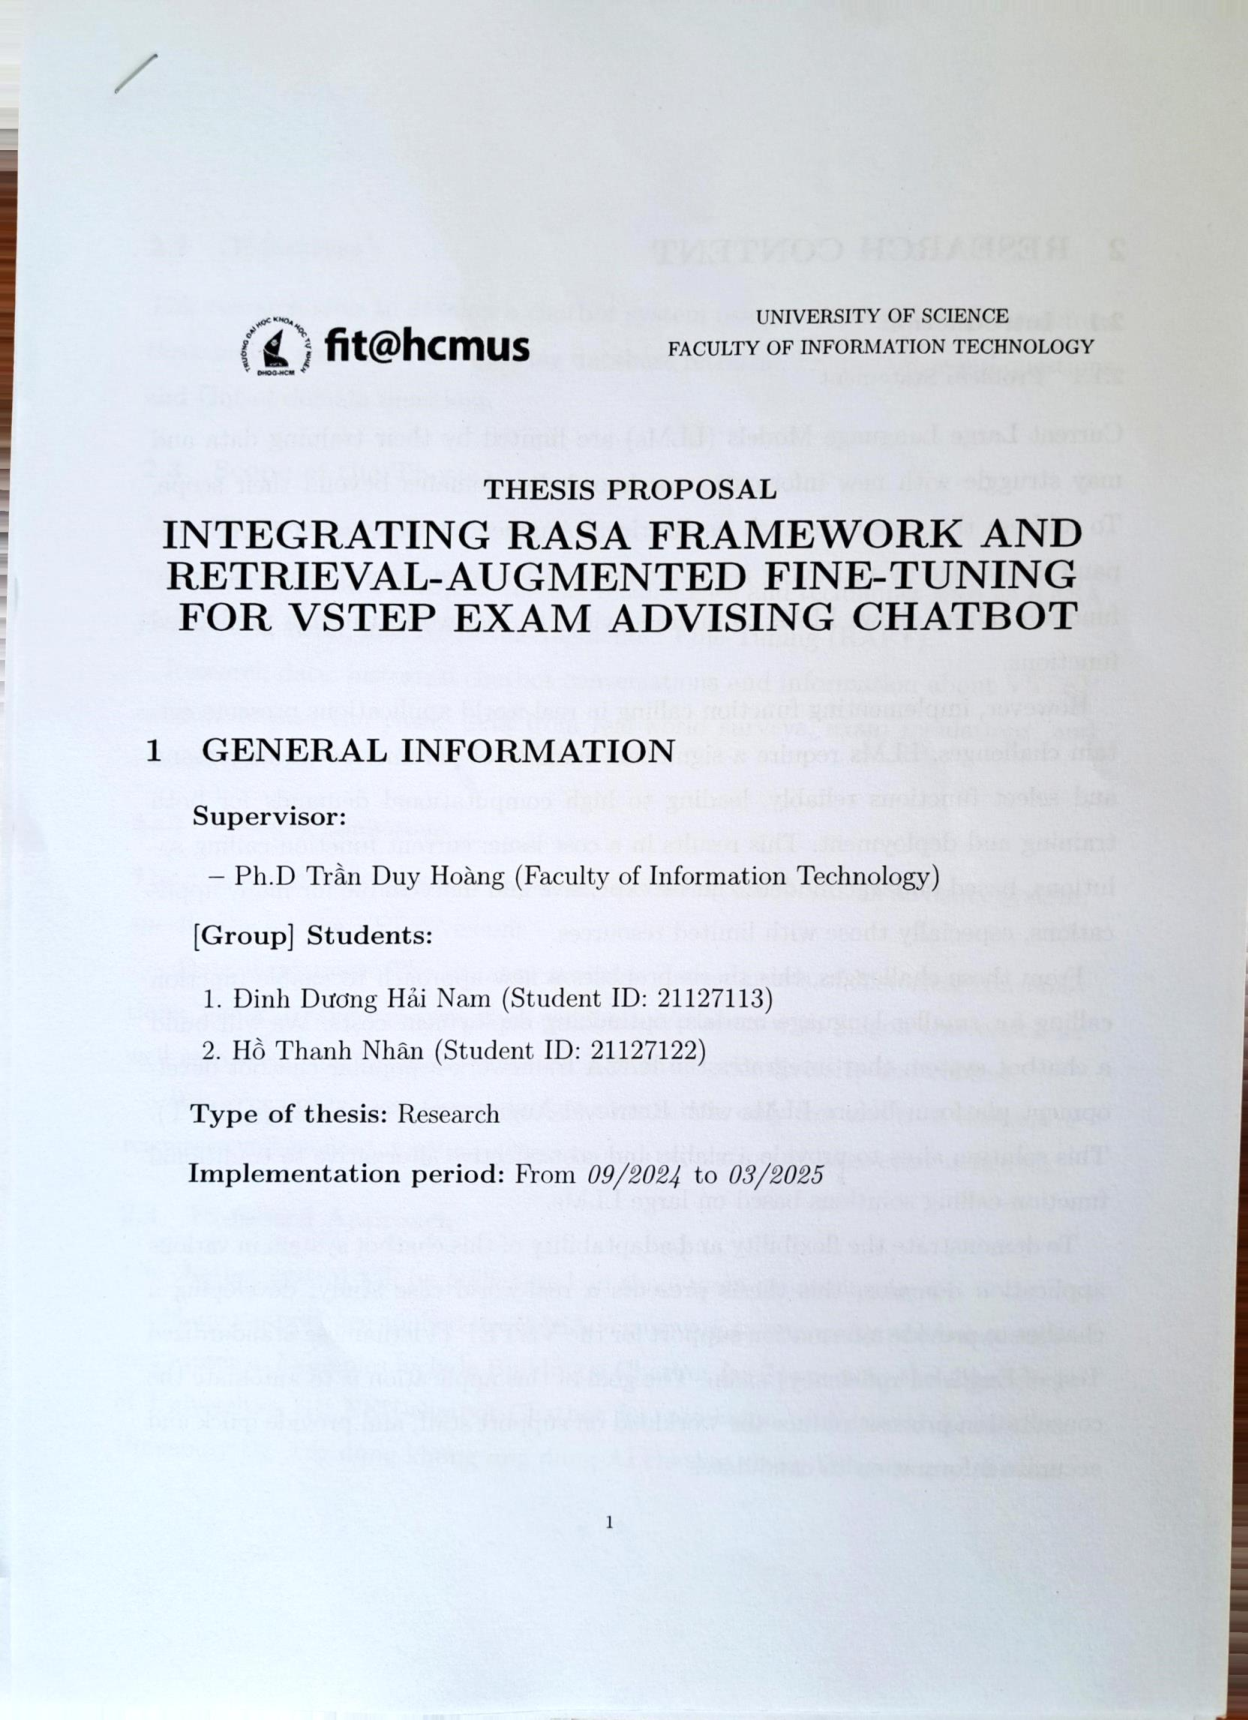
\includepdf[pages=-]{Appendix/Proposal.pdf}

\setcounter{page}{2}
% Mục lục, danh sách hình, danh sách bảng
\addcontentsline{toc}{chapter}{Mục lục}

\tableofcontents

%\listoffigures
\cleardoublepage
\phantomsection
\addcontentsline{toc}{chapter}{\listfigurename}
\listoffigures

\cleardoublepage
\phantomsection
\addcontentsline{toc}{chapter}{\listtablename}
\listoftables
%\listoftables

\cleardoublepage
\phantomsection
\addcontentsline{toc}{chapter}{Tóm tắt}
\chapter*{Tóm tắt}
\label{summary}

Trong bối cảnh dữ liệu tri thức ngày càng phát triển theo thời gian, Đồ thị Tri thức Thời gian (Temporal Knowledge Graphs - TKGs) đóng vai trò quan trọng trong việc biểu diễn các mối quan hệ động giữa các thực thể. Tuy nhiên, bài toán Suy luận Đồ thị Tri thức Thời gian (TKGR) vẫn đối mặt với nhiều thách thức: các phương pháp hiện tại chưa khai thác hiệu quả thông tin lịch sử bậc cao, gặp hạn chế trong xử lý khối lượng dữ liệu lớn và thiếu tính giải thích trong quá trình suy luận. Mặc dù sự xuất hiện của các Mô hình Ngôn ngữ Lớn (LLMs) mở ra tiềm năng mới, việc ứng dụng chúng vào TKGR vẫn bị cản trở bởi các chiến lược prompt đơn giản và thiếu khả năng tùy chỉnh theo truy vấn.

Nghiên cứu này đề xuất phương pháp MSKGen (Multi-Source Knowledge-Based Generation) - một cách tiếp cận mới kết hợp tri thức đa nguồn để giải quyết các hạn chế trên. Phương pháp của chúng tôi tích hợp ba thành phần chính: (1) Trích xuất quy tắc logic thời gian thông qua kỹ thuật temporal random walks và tinh chỉnh bằng LLMs, (2) Truy xuất tri thức ngữ nghĩa sử dụng cơ sở dữ liệu vector hóa kết hợp kỹ thuật RAG, và (3) Cơ chế lập luận đa nguồn hướng dẫn bởi truy vấn. Hệ thống đánh giá kết quả thông qua sự kết hợp giữa điểm số từ LLMs và mô hình đồ thị được huấn luyện trước.

Kết quả thực nghiệm trên các tập dữ liệu cho thấy MSKGen vượt trội so với các phương pháp tiên tiến hiện tại. Phương pháp này không chỉ nâng cao độ chính xác mà còn cung cấp khả năng giải thích quá trình suy luận thông qua việc kết hợp các quy tắc logic và tri thức ngữ nghĩa. Ứng dụng tiềm năng của MSKGen bao gồm dự đoán xu hướng kinh tế, hỗ trợ ra quyết định y tế và nâng cao hiệu suất của hệ thống khuyến nghị động, mở ra hướng nghiên cứu mới về tích hợp LLMs vào các bài toán đồ thị tri thức phức tạp.


\cleardoublepage
\phantomsection
\addcontentsline{toc}{chapter}{Danh sách các từ viết tắt}
\chapter*{Danh sách các từ viết tắt}

\begin{acronym}[LONGEST]
    \acro{AI}{Artificial Intelligence}
    \acro{AIML}{Artificial Intelligence Markup Language}
    \acro{ALICE}{Artificial Linguistic Internet Computer Entity}
    \acro{API}{Application Programming Interface}
    \acro{BERT}{Bidirectional Encoder Representations from Transformers}
    \acro{CCCD}{Căn cước công dân (Citizen ID)}
    \acro{CEFR}{Common European Framework of Reference for Languages}
    \acro{CoT}{Chain-of-Thought}
    \acro{CRQA}{Crowd-powered Real-time Question Answering}
    \acro{DB}{Database}
    \acro{DIET}{Dual Intent and Entity Transformer}
    \acro{DM}{Dialogue Management}
    \acro{DSF}{Domain-Specific Fine-tuning}
    \acro{FAQ}{Frequently Asked Questions}
    \acro{FN}{False Negative}
    \acro{FP}{False Positive}
    \acro{GPT}{Generative Pre-training Transformer}
    \acro{HCI}{Human-Computer Interaction}
    \acro{HF}{Hugging Face}
    \acro{IBM}{International Business Machines Corporation}
    \acro{ID}{Identity document}
    \acro{IELTS}{International English Language Testing System}
    \acro{LDA}{Latent Dirichlet
 Allocation}
    \acro{LLM}{Large Language Model}
    \acro{NER}{Named Entity Recognition}
    \acro{NEU}{National Economics University}
    \acro{NLP}{Natural Language Processing}
    \acro{NLU}{Natural Language Understanding}
    \acro{OOD}{Out-of-Distribution}
    \acro{\detokenize{Q&A}}{Question and Answer}
    \acro{RAFT}{Retrieval-Augmented Fine-Tuning}
    \acro{RAG}{Retrieval-Augmented Generation}
    \acro{Regex}{Regular Expression}
    \acro{SFT}{Supervised Fine-Tuning}
    \acro{STT}{speech-to-text}
    \acro{TED}{Transformer Embedding Dialogue}
    \acro{TN}{True Negative}
    \acro{TP}{True Positive}
    \acro{TOEFL}{Test of English as a Foreign Language}
    \acro{TTS}{text-to speech}
    \acro{URL}{Uniform Resource Locator}
    \acro{VND}{Viet Nam Dong}
    \acro{VSTEP}{Vietnamese Standardized Test of English Proficiency}
    \acro{XAI}{Explainable Artificial Intelligent}
\end{acronym}

\clearpage

\pagenumbering{arabic} % Đánh số 1, 2, 3, ...

% Các chương nội dung
\chapter{GIỚI THIỆU}
\label{Chapter1}

Chương đầu tiên của khóa luận sẽ trình bày một cách hệ thống các khái
niệm cơ bản liên quan đến vấn đề được nghiên cứu, bao gồm mô tả về đồ
thị tri thức thời gian, bài toán dự đoán liên kết, cũng như những ứng dụng thực tiễn và khoa học của cấu trúc dữ liệu này. Tiếp theo, khóa luận chỉ ra các thách thức trong bài toán đang thực hiện và cung cấp một cái nhìn tổng quan về các hướng giải quyết cho bài toán đang thực hiện, đồng thời phân tích những hạn chế và thách thức tồn tại trong từng phương pháp hiện có. Trên cơ sở đó, khóa luận sẽ giới thiệu phương pháp tiếp cận được lựa chọn để giải quyết vấn đề nghiên cứu. Cuối cùng, chương sẽ tóm tắt những đóng góp chính của khóa luận và đưa ra sơ đồ bố cục cho toàn bộ nội dung đề tài.


\section{Giới thiệu tổng quan}

Năm 2012, Google giới thiệu công cụ tìm kiếm tích hợp đồ thị tri thức (Knowledge Graph - KG) \cite{ref_article01}, một cấu trúc dữ liệu do E.W. Schneider đề xuất từ năm 1973 \cite{ref_article24}. Sự kiện này đã thu hút sự chú ý của các tập đoàn công nghệ khác như Facebook, IBM và Microsoft \cite{ref_article25}, họ nhanh chóng nhận ra tiềm năng của đồ thị tri thức trong việc ứng dụng vào các hệ thống của mình. Bằng việc mô hình hóa các thực thể đại diện cho sự vật, hiện tượng bằng các nút và biểu diễn các mối quan hệ giữa chúng trong thế giới thực qua các cạnh, đồ thị tri thức có khả năng hiểu, dễ dàng tích hợp, trích xuất cũng như tổ chức lượng lớn dữ liệu cực kỳ dễ dàng. Những ưu điểm này đã thúc đẩy sự phát triển của các dự án mã nguồn mở về cơ sở tri thức nổi tiếng như Wikidata \cite{ref_article26} và YAGO \cite{ref_article21}. Ngoài ra, đồ thị tri thức còn được ứng dụng vào nhiều lĩnh vực nhận biết tri thức (knowledge-aware), tạo nên các ứng dụng như hệ thống gợi ý, tìm kiếm ngữ nghĩa và hệ thống trả lời câu hỏi. Điều này đã khẳng định vị thế của đồ thị tri thức trong lĩnh vực biểu diễn tri thức nói riêng và trí tuệ nhân tạo nói chung.

\begin{figure}[htp]
\centering
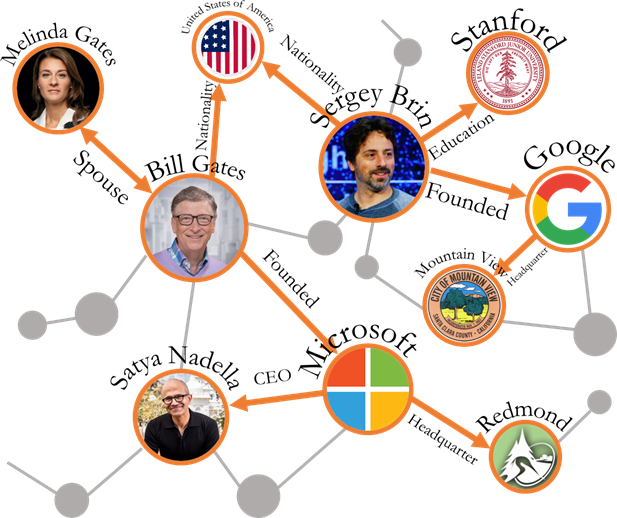
\includegraphics[width=15cm]{images/KGexample1.png}
\caption{Đồ thị tri thức với các thực thể như cá nhân, tổ chức, địa điểm và quốc gia được kết nối qua các mối quan hệ như sáng lập, quốc tịch, học vấn, trụ sở và vai trò lãnh đạo.
Các nút đại diện cho thực thể nổi bật (Bill Gates, Sergey Brin, Microsoft, Google...) và các cạnh có hướng thể hiện rõ ràng loại quan hệ giữa chúng.}
\label{fig:chatbots_classification}
\end{figure}

Mặc dù đồ thị tri thức là một công cụ mạnh mẽ cho việc tổ chức và xử lý kiến thức, chúng thường bị giới hạn trong một không gian tĩnh mà ở đó các nút và cạnh không phát triển theo diễn biến thời gian. Hạn chế này vô tình khiến đồ thị tri thức thiếu đi khả năng phản ánh sự biến đổi của thế giới thực, nơi mà sự liên kết giữa các thực thể có thể được hình thành hay mất đi qua từng thời điểm khác nhau. Ví dụ, quan sát đồ thị tri thức tĩnh trong hình minh họa, ta có thể thấy các mối quan hệ như "Bill Gates - Founded - Microsoft" hoặc "Sergey Brin - Founded - Google" được biểu diễn mà không có thông tin thời gian cụ thể. Điều này dẫn đến việc không thể xác định được rằng Bill Gates thành lập Microsoft vào năm 1975, hay Sergey Brin đồng sáng lập Google vào năm 1996. Hơn nữa, với lượng thông tin ngày càng lớn và phức tạp như hiện tại, việc thiếu yếu tố thời gian khiến cho các hệ thống dựa trên đồ thị tri thức tĩnh không thể nắm bắt được sự thay đổi của các mối quan hệ theo thời gian, dẫn đến thông tin lỗi thời và không chính xác cho các ứng dụng thực tế.

Để giải quyết vấn đề này, đồ thị tri thức thời gian (Temporal Knowledge Graph - TKG)~\cite{ref_article02} được đề xuất với ý tưởng chính là bổ sung một chiều thời gian vào cấu trúc bộ ba (thực thể đầu, quan hệ, thực thể đuôi) ban đầu. Lúc này, bộ ba sẽ mở rộng thành bộ bốn (thực thể đầu, quan hệ, thực thể đuôi, nhãn thời gian) và tri thức được mã hóa thành (Bill Gates, Founded, Microsoft, 1975) hoặc (Sergey Brin, Founded, Google, 1996). Việc tích hợp thêm trường thời gian giúp cho đồ thị tri thức nắm bắt sự thay đổi, mang đến khả năng diễn đạt và xử lý kiến thức một cách linh hoạt hơn, phù hợp hơn với bản chất động của thế giới thực.

\begin{figure}[h!]
\centering
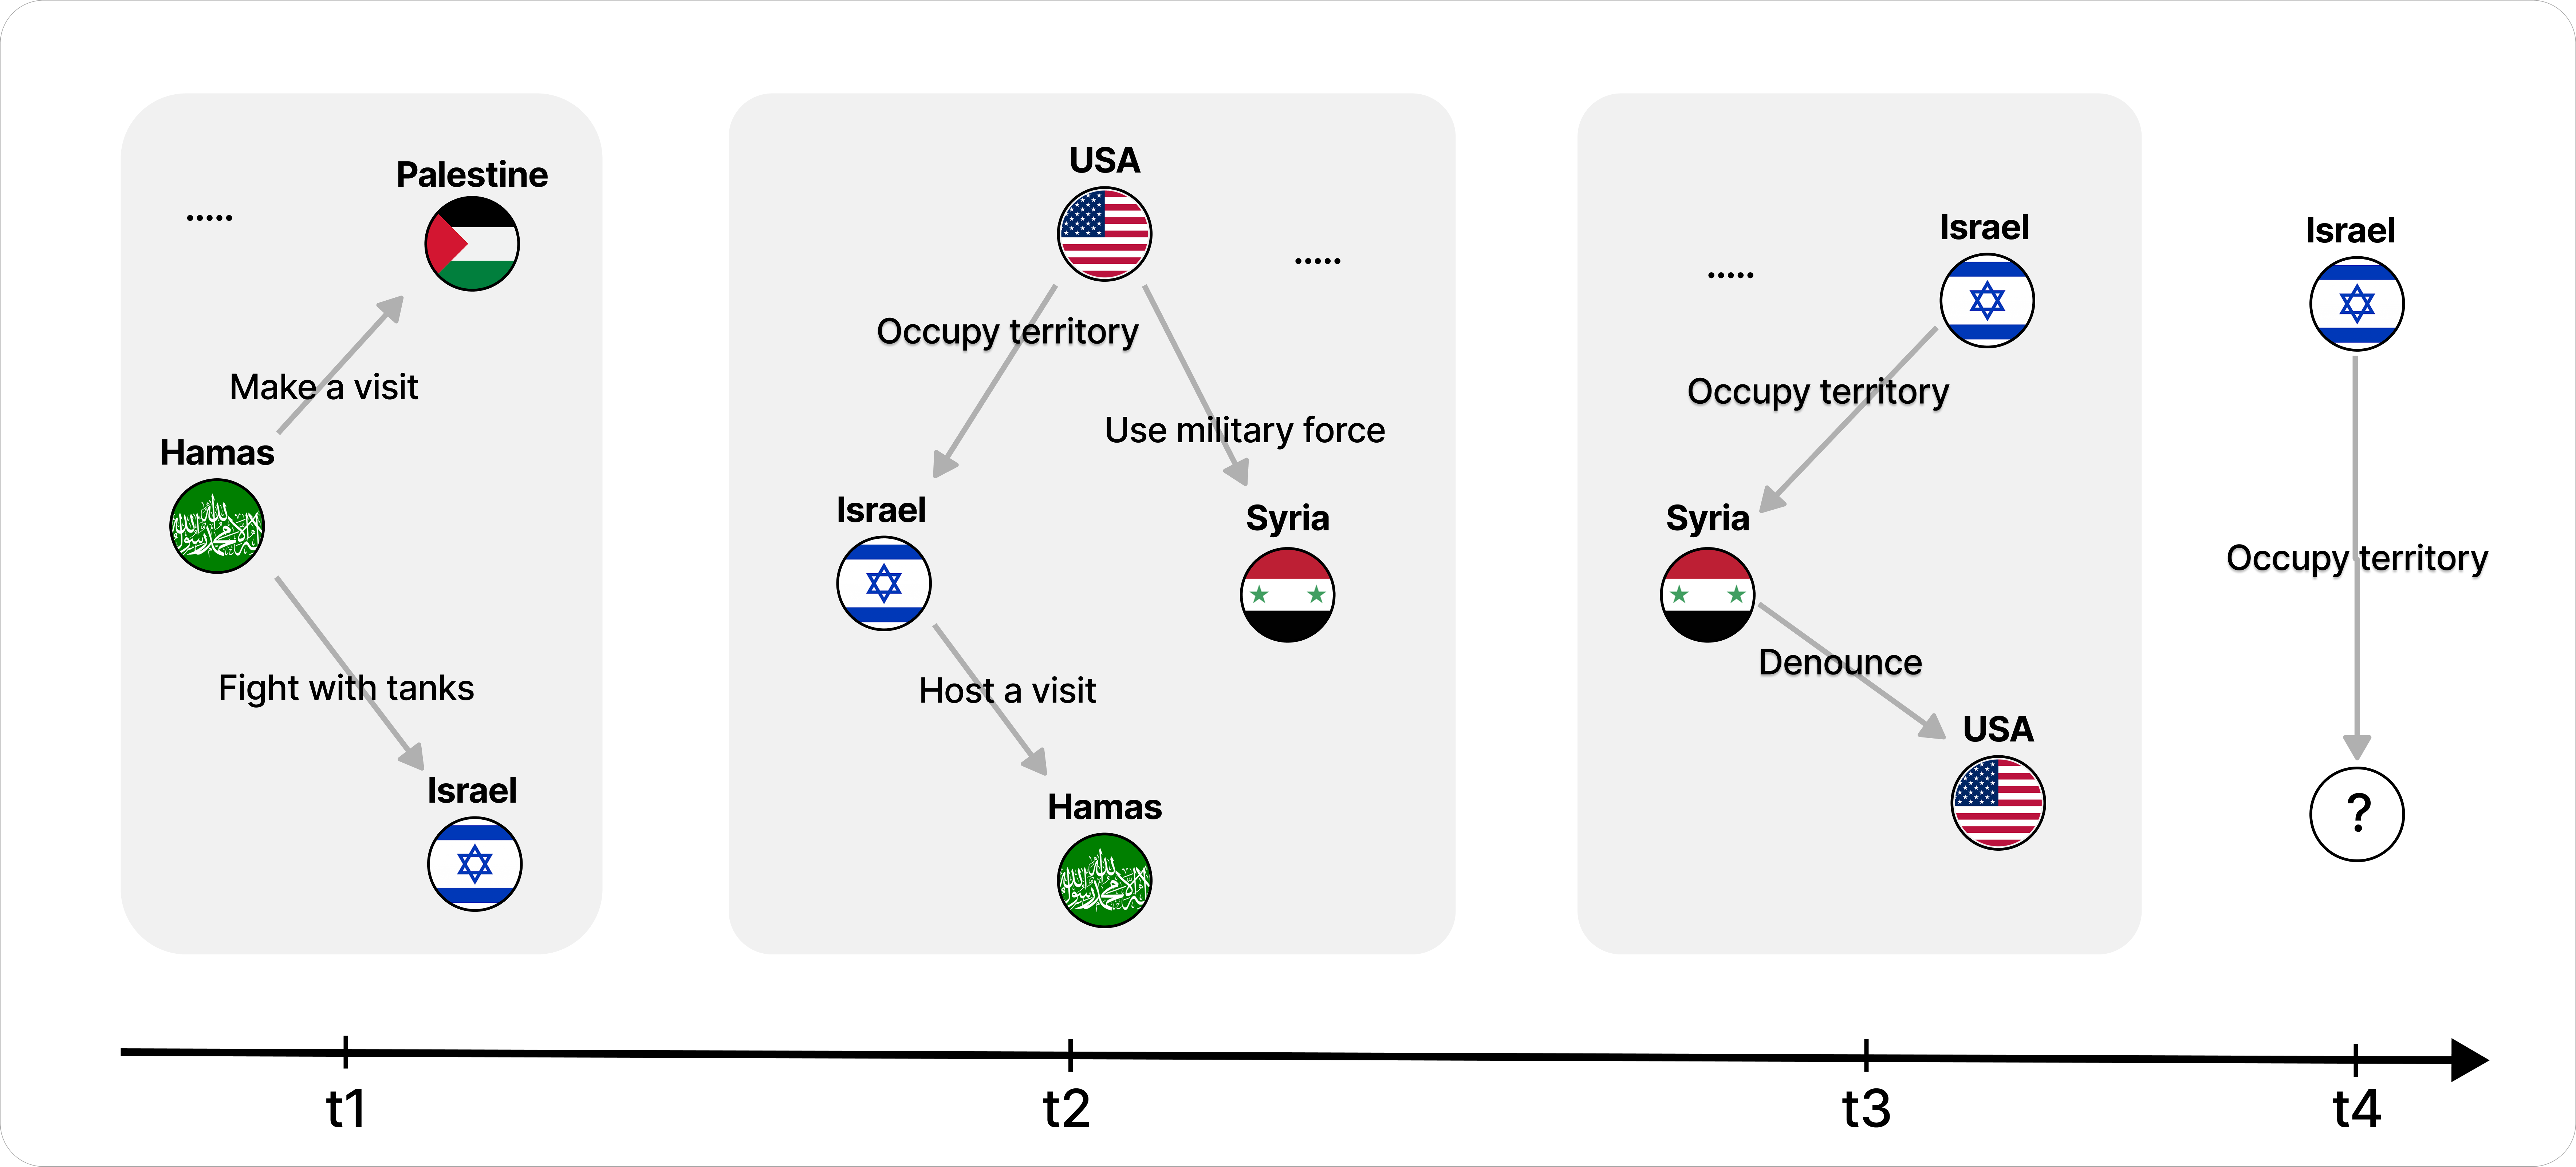
\includegraphics[width=15cm]{images/TKGexample1.png}
\caption{Hình ảnh minh họa quá trình dự đoán sự kiện tương lai trên Đồ thị Tri thức Thời gian (Temporal Knowledge Graph - TKG). Tại mỗi thời điểm $t_1, t_2, t_3$, các sự kiện giữa các thực thể như Israel, Hamas, USA, Syria... được biểu diễn dưới dạng các bộ tứ (subject, relation, object, timestamp). Dựa trên chuỗi sự kiện lịch sử này, mô hình TKGR sẽ sử dụng các quan hệ và tương tác trong quá khứ để dự đoán đối tượng (object) tiếp theo của chủ thể (subject) Israel với quan hệ "Occupy territory" tại thời điểm $t_4$. Quá trình này thể hiện khả năng suy luận và dự báo sự kiện tương lai dựa trên mẫu quan hệ động trong quá khứ của đồ thị tri thức thời gian.}
\label{fig:chatbots_classification}
\end{figure}

Cả đồ thị tri thức tĩnh và đồ thị tri thức thời gian đều được xây dựng từ nhiều nguồn dữ liệu mở với quy mô lớn (ví dụ GDELT \cite{ref_article20}, YAGO \cite{ref_article21}), tuy nhiên, chúng đều gặp phải vấn đề chung về tính bất hoàn thiện. Tính bất hoàn thiện này thể hiện ở việc các tri thức giá trị trong đồ thị tri thức thời gian thường bị mất đi các thực thể, mối quan hệ, thông tin thời gian hoặc thậm chí là bộ bốn dữ kiện bị ẩn hoàn toàn. Hệ quả là các ứng dụng dưới dòng bị hạn chế về độ chính xác do không thể tạo ra các kết nối quan trọng cho thông tin được truy vấn, dẫn đến các giả định sai lệch so với thực tế.

Bài toán suy luận trên đồ thị tri thức thời gian (Temporal Knowledge Graph Reasoning - TKGR) nhằm giải quyết vấn đề này bằng cách dự đoán các sự kiện mới dựa trên thông tin lịch sử có sẵn. Nghiên cứu hiện nay cho thấy rằng các mô hình TKGR có thể được chia làm hai nhánh chính là suy luận dựa trên nội suy và suy luận dựa trên ngoại suy. Với nội suy, các kỹ thuật ở nhánh này dự đoán các dữ kiện mới bằng việc phân tích và khai thác các đặc trưng của dữ kiện đã có trong TKGs, các phương pháp như phân rã ten-xơ (Tensor Decomposition) và chuyển vị quan hệ thời gian (Time-Aware Relation Transformation) nổi bật trong nhánh này do độ chính xác cao. Với ngoại suy, các kỹ thuật sẽ chú trọng vào tính phát triển của dữ liệu qua thời gian để dự đoán các dữ kiện nằm bên ngoài tập dữ liệu, nhằm dự đoán những sự kiện trong tương lai, các hướng giải quyết là mạng nơ-ron đồ thị thời gian (Temporal Graph Neural Networks) và suy tập luật thời gian (Temporal Rule Induction) xuất hiện nhiều trong nghiên cứu gần đây từ nhánh này.

Cả hai nhánh tiếp cận đều có những ưu điểm riêng trong việc tích hợp thông tin thời gian vào mô hình. Tuy nhiên, trong phạm vi của đề tài này, chúng tôi lựa chọn phương pháp tích hợp tri thức đa nguồn trong nhánh tiếp cận ngoại suy để giải quyết bài toán suy luận đồ thị tri thức thời gian. Lý do là phương pháp này có khả năng dự đoán các sự kiện tương lai bằng cách tận dụng sức mạnh của các mô hình ngôn ngữ lớn (LLMs)~\cite{ref_article04} trong việc hiểu ngữ nghĩa và suy luận phức tạp, đồng thời có thể xử lý được các truy vấn linh hoạt theo từng ngữ cảnh cụ thể.

Đặc biệt, sự xuất hiện của các LLMs như GPT~\cite{ref_article05}, LLaMA~\cite{ref_article06}, và DeepSeek~\cite{ref_article07} đã mở ra những cơ hội mới cho TKGR nhờ khả năng xử lý ngữ nghĩa và suy luận vượt trội. Các mô hình này có thể hiểu được các mối liên kết ngữ nghĩa phức tạp và các mẫu thời gian trong dữ liệu, mang lại tiềm năng giải quyết những thách thức về tính giải thích trong TKGR~\cite{ref_article03}. Chính vì vậy, đề tài này tập trung vào việc phát triển phương pháp MSKGen (Multi-Source Knowledge-Based Generation), một cách tiếp cận mới cho TKGR dựa trên việc tích hợp tri thức đa nguồn và tùy chỉnh theo truy vấn, nhằm tận dụng tối đa khả năng của LLMs trong việc dự đoán các sự kiện tương lai một cách chính xác và có tính giải thích cao.


\section{Thách thức của bài toán}

\subsection{Hạn chế trong khai thác ngữ nghĩa của LLMs}
Các phương pháp hiện tại ứng dụng LLMs vào TKGR chủ yếu tập trung vào kỹ thuật prompt engineering đơn giản mà chưa tận dụng hết tiềm năng hiểu ngữ nghĩa sâu của mô hình. Việc phụ thuộc vào các phương pháp truy xuất truyền thống dựa trên khớp lược đồ (schema matching) dẫn đến việc bỏ qua các mối quan hệ ngữ nghĩa tiềm ẩn trong dữ liệu lịch sử. Ví dụ, khi dự đoán sự kiện "công ty A hợp tác với công ty B", các phương pháp hiện tại chỉ xem xét các sự kiện trực tiếp liên quan đến hai công ty này mà không nhận biết được mối liên hệ gián tiếp thông qua các thực thể trung gian hoặc ngữ cảnh thời gian mở rộng. Điều này làm giảm khả năng phát hiện các khuôn mẫu phức tạp và quan hệ đa tầng trong TKGs.

\subsection{Thiếu tính cá nhân hóa trong suy luận}
Các hệ thống TKGR hiện có thường áp dụng cùng một chiến lược suy luận cho mọi truy vấn mà không xem xét đặc thù ngữ nghĩa của từng yêu cầu cụ thể. Việc không phân biệt được sự khác biệt giữa các loại truy vấn (ví dụ: truy vấn về sự kiện kinh tế vs. sự kiện chính trị) dẫn đến việc tạo ra các phản hồi chung chung. Hệ quả là các dự đoán thiếu tính chính xác cục bộ và không phản ánh được sắc thái thời gian đặc thù của từng sự kiện. Nghiêm trọng hơn, các phương pháp dựa trên LLMs hiện tại thường không xử lý được các truy vấn yêu cầu kết hợp nhiều nguồn tri thức đa dạng.

\subsection{Khó khăn trong xử lý thông tin thời gian đa tầng}
TKGs chứa các mối quan hệ thời gian ở nhiều mức độ phức tạp khác nhau, từ các sự kiện đơn lẻ (event-level) đến các xu hướng dài hạn (trend-level). Các phương pháp hiện tại gặp khó khăn trong việc đồng thời xử lý:
\begin{itemize}
    \item Thông tin lịch sử bậc cao (high-order dependencies) giữa các sự kiện cách biệt về thời gian
    \item Tương tác phi tuyến tính giữa các yếu tố thời gian ngắn hạn và dài hạn
    \item Sự mâu thuẫn tiềm ẩn giữa các nguồn tri thức khác nhau
\end{itemize}

\subsection{Giới hạn trong tích hợp tri thức đa nguồn}
Phần lớn các phương pháp TKGR hiện nay chỉ tập trung vào khai thác thông tin từ cấu trúc đồ thị mà bỏ qua các nguồn tri thức bổ sung như văn bản phi cấu trúc, cơ sở dữ liệu quan hệ, hay tri thức miền chuyên gia. Sự thiếu hụt này dẫn đến hai hệ quả chính: (1) Các dự đoán không thể tận dụng được thông tin ngữ cảnh phong phú từ các nguồn dữ liệu đa phương thức, (2) Hệ thống khó duy trì tính nhất quán khi xử lý các truy vấn đòi hỏi tích hợp tri thức liên ngành.

\subsection{Thách thức về tính giải thích}
Mặc dù LLMs có khả năng suy luận phức tạp, các phương pháp TKGR hiện tại chưa cung cấp được cơ chế giải thích rõ ràng cho từng dự đoán. Việc thiếu minh bạch trong quá trình ra quyết định đặc biệt nghiêm trọng trong các ứng dụng nhạy cảm như dự báo tài chính hoặc chẩn đoán y tế, nơi cần theo dõi được logic suy luận và nguồn gốc của từng dự đoán. Hơn nữa, sự phụ thuộc quá mức vào các mô hình hộp đen (black-box models) làm hạn chế khả năng hiệu chỉnh và tối ưu hệ thống.


\section{Động lực và hướng tiếp cận}

\subsection{Động lực nghiên cứu}
Các phương pháp hiện tại trong suy luận đồ thị tri thức thời gian (TKGR) chủ yếu dựa trên các mô hình học sâu với ba hạn chế chính: (1) Thiếu tính giải thích do sử dụng kiến trúc "hộp đen", (2) Phụ thuộc quá mức vào thông tin lịch sử bậc nhất mà bỏ qua các mối quan hệ đa tầng, và (3) Khả năng tùy biến thấp trước các truy vấn cụ thể. Ví dụ, khi dự đoán sự kiện "Công ty A hợp tác chiến lược với Công ty B", các phương pháp truyền thống chỉ xem xét các sự kiện trực tiếp giữa hai thực thể này mà bỏ qua các yếu tố ngữ cảnh như mối quan hệ gián tiếp qua đối tác phụ hoặc xu hướng dài hạn trong lịch sử hợp tác.

Sự xuất hiện của các mô hình ngôn ngữ lớn (LLMs) mở ra cơ hội cải thiện TKGR thông qua khả năng hiểu ngữ nghĩa sâu và suy luận logic. Tuy nhiên, việc áp dụng LLMs vào TKGR hiện nay vẫn chưa khai thác hết tiềm năng do: (1) Chiến lược prompt đơn giản không tận dụng được cấu trúc thời gian phức tạp, (2) Thiếu cơ chế tích hợp tri thức từ nhiều nguồn đa dạng, và (3) Không cân bằng được giữa độ chính xác và tính giải thích. Điều này dẫn đến các dự đoán thiếu tin cậy trong các ứng dụng thực tế như dự báo tài chính hoặc phân tích chính trị.

\subsection{Hướng tiếp cận}
Phương pháp MSKGen được thiết kế để giải quyết các thách thức trên thông qua ba trụ cột chính:

1. \textbf{Trích xuất tri thức dựa trên quy tắc thời gian}: Sử dụng "temporal random walks" \cite{ref_article28} để khám phá các mẫu quan hệ động trong dữ liệu lịch sử. Quy trình bao gồm: (a) Lấy mẫu các chuỗi sự kiện tuân thủ ràng buộc thời gian, (b) Đánh giá chất lượng quy tắc bằng độ đo Kulczynski \cite{ref_article16}, (c) Tinh chỉnh quy tắc thông qua tương tác với LLMs. Ví dụ, từ chuỗi sự kiện "A hợp tác với B → B đầu tư vào C → C mở rộng thị trường", hệ thống có thể rút ra quy tắc logic về chuỗi tác động kinh tế.

2. \textbf{Truy xuất tri thức ngữ nghĩa đa nguồn}: Áp dụng kỹ thuật RAG (Retrieval-Augmented Generation) \cite{ref_article27} và hệ thống cơ sở dữ liệu vector Chroma \cite{ref_article17} để tìm kiếm các sự kiện tương đồng ngữ nghĩa, cho phép phát hiện các mối quan hệ tiềm ẩn không được biểu diễn tường minh trong đồ thị.

3. \textbf{Lập luận đa nguồn có hướng dẫn}: Kết hợp đầu ra từ hai quy trình trên thông qua cơ chế điều phối động: (a) Phân tích cú pháp và ngữ nghĩa của truy vấn để xác định trọng số cho từng nguồn tri thức, (b) Sử dụng LLMs để tổng hợp thông tin dưới dạng các chuỗi suy luận có cấu trúc, (c) Đánh giá độ tin cậy dựa trên sự nhất quán giữa các nguồn. Ví dụ, khi dự đoán xu hướng thị trường, hệ thống sẽ cân bằng giữa quy tắc thống kê từ dữ liệu lịch sử và phân tích ngữ cảnh từ báo cáo kinh tế.

Khác biệt cốt lõi của MSKGen so với các phương pháp trước đây nằm ở khả năng thích ứng động với từng truy vấn cụ thể thông qua việc tích hợp: (1) Logic thời gian từ các quy tắc được học, (2) Bối cảnh ngữ nghĩa từ RAG, và (3) Khả năng suy luận đa tầng của LLMs. Sự kết hợp này không chỉ cải thiện độ chính xác mà còn tạo ra các lộ trình suy luận có thể giải thích được, đáp ứng yêu cầu của các ứng dụng thực tế yêu cầu tính minh bạch cao.

\section{Mục tiêu và đóng góp của đề tài}

\subsection{Mục tiêu đề tài}
Mục tiêu chung của đề tài khóa luận tốt nghiệp này là nghiên cứu và phát triển phương pháp suy luận hiệu quả trên đồ thị tri thức thời gian ở nhánh bài toán ngoại suy, tập trung vào việc dự đoán các sự kiện tương lai dựa trên chuỗi sự kiện lịch sử. Mục tiêu cụ thể bao gồm:

• Tổng hợp và phân tích các công trình nghiên cứu trong và ngoài nước về bài toán suy luận đồ thị tri thức thời gian, đặc biệt là các phương pháp ứng dụng mô hình ngôn ngữ lớn vào TKGR nhằm khảo sát các xu hướng và tiến triển của lĩnh vực.

• Phân tích sâu các thách thức và hạn chế của các phương pháp hiện tại trong việc tích hợp tri thức đa nguồn và tùy chỉnh suy luận theo truy vấn cụ thể. Từ đó đề xuất hướng giải quyết khả quan cho nhánh bài toán ngoại suy thông qua việc kết hợp kỹ thuật trích xuất quy tắc và truy xuất ngữ nghĩa.

• Thiết kế và triển khai framework MSKGen, một phương pháp mới tích hợp tri thức từ nhiều nguồn khác nhau để nâng cao độ chính xác và tính giải thích trong dự đoán sự kiện tương lai trên đồ thị tri thức thời gian.

• Thực nghiệm và đánh giá hiệu suất của mô hình MSKGen trên các bộ dữ liệu chuẩn, so sánh với các phương pháp tiên tiến hiện có để chứng minh tính hiệu quả và khả năng ứng dụng thực tế của phương pháp đề xuất.

\subsection{Đóng góp của đề tài}
Những đóng góp chính của đề tài nghiên cứu này bao gồm:

• Giới thiệu MSKGen, một framework tiên tiến cho suy luận đồ thị tri thức thời gian theo truy vấn cụ thể thông qua tích hợp tri thức đa nguồn. Phương pháp này kết hợp khả năng trích xuất quy tắc logic chất lượng cao từ dữ liệu lịch sử với kỹ thuật truy xuất ngữ nghĩa, đảm bảo cả tính chính xác lẫn độ sâu ngữ nghĩa trong quá trình suy luận.

• Phát triển cơ chế suy luận nhận biết truy vấn (query-aware reasoning) có khả năng tùy chỉnh quá trình dự đoán theo đặc thù của từng yêu cầu cụ thể. Cơ chế này tận dụng kỹ thuật Retrieval-Augmented Generation để thu thập ngữ cảnh phong phú từ các nguồn dữ kiện đa dạng, nâng cao chất lượng và độ tin cậy của dự đoán.

• Tối ưu hóa khả năng xử lý của mô hình ngôn ngữ lớn trong việc kết nối các dữ kiện có cấu trúc đa dạng và tích hợp thông tin tương tự về mặt ngữ nghĩa. Điều này cho phép MSKGen tạo ra các câu trả lời phù hợp với từng truy vấn cụ thể trong khi tối đa hóa tiềm năng hiểu ngữ nghĩa của LLMs.

• Đánh giá toàn diện trên các tập dữ liệu chuẩn cho thấy MSKGen vượt trội đáng kể so với các phương pháp hiện có về độ chính xác dự đoán sự kiện, đồng thời duy trì tính giải thích cao thông qua việc kết hợp tri thức từ nhiều nguồn khác nhau.

\subsection{Bố cục trình bày}
Khóa luận được tổ chức thành sáu chương với các nội dung được tóm tắt như sau:

• Chương 1: Trình bày tổng quan về vấn đề đang được nghiên cứu, bao gồm giới thiệu về đồ thị tri thức thời gian và bài toán suy luận TKGR. Chương này phân tích các thách thức hiện tại của bài toán, từ đó chỉ ra động lực, hướng tiếp cận, mục tiêu cũng như đóng góp của khóa luận.

• Chương 2: Tập trung vào việc khảo sát và phân tích các công trình nghiên cứu liên quan đến suy luận đồ thị tri thức thời gian, đặc biệt là các phương pháp ứng dụng mô hình ngôn ngữ lớn. Thông qua phân tích ưu điểm và hạn chế của từng phương pháp, chương này làm rõ cơ sở lựa chọn hướng tiếp cận của nghiên cứu.

• Chương 3: Cung cấp nền tảng lý thuyết và các khái niệm cơ bản làm cơ sở cho phương pháp đề xuất. Nội dung bao gồm định nghĩa chính thức về đồ thị tri thức thời gian, bài toán suy luận TKGR, các kỹ thuật mô hình ngôn ngữ lớn và Retrieval-Augmented Generation.

• Chương 4: Giới thiệu chi tiết framework MSKGen, bao gồm kiến trúc tổng thể, các thành phần chính và cơ chế hoạt động. Chương này trình bày phương pháp trích xuất quy tắc thời gian, kỹ thuật truy xuất ngữ nghĩa và cơ chế suy luận tích hợp đa nguồn.

• Chương 5: Trình bày kết quả thực nghiệm toàn diện của MSKGen trên các tập dữ liệu chuẩn, so sánh hiệu suất với các phương pháp tiên tiến hiện có. Chương này cũng phân tích ảnh hưởng của các siêu tham số và thành phần khác nhau đến hiệu suất của mô hình.

• Chương 6: Tóm tắt các kết quả đạt được, đánh giá mức độ hoàn thành mục tiêu đề ra và đề xuất các hướng nghiên cứu tiềm năng trong tương lai dựa trên những hạn chế và cơ hội mở ra từ nghiên cứu này.


\chapter{CÁC CÔNG TRÌNH \\ LIÊN QUAN}
\label{Chapter2}

Chương này tập trung vào việc giới thiệu các mô hình tiên tiến cho bài toán dự đoán liên kết trong đồ thị tri thức thời gian, được phân loại thành hai nhánh giải quyết chính là nội suy và ngoại duy được giới thiệu ở chương 1. Để đảm bảo tính rõ ràng và thống nhất trong toàn bộ khóa luận cũng như các phần tiếp theo, Bảng 2.1 tóm tắt các ký hiệu được sử dụng. Nhiệm vụ dự đoán các thành phần bị thiếu trong đồ thị tri thức thời gian, cho dù chúng nằm trong hay ngoài tập dữ liệu hiện có, đã dẫn đến sự phân biệt hai phương pháp chính: Hoàn thiện dựa trên nội suy và
Hoàn thiện dựa trên ngoại suy. Các phương pháp này sẽ được trình bày ở các mục con tương ứng trong nội dung tiếp theo.


\section{Tóm tắt các ký hiệu và định nghĩa chung}

Trong nghiên cứu về suy luận đồ thị tri thức thời gian, việc thiết lập một hệ thống ký hiệu nhất quán và rõ ràng đóng vai trò quan trọng trong việc trình bày các khái niệm và phương pháp một cách chính xác. Hệ thống ký hiệu được sử dụng trong nghiên cứu này được xây dựng dựa trên các tiêu chuẩn quốc tế và phù hợp với các nghiên cứu tiền phong trong lĩnh vực đồ thị tri thức thời gian.

Đồ thị tri thức thời gian được định nghĩa là một chuỗi các snapshot có dấu thời gian \( G = \{G_1, G_2, ..., G_t, ...\} \), trong đó mỗi snapshot \( G_t = (\mathcal{E}, \mathcal{R}, \mathcal{T}) \) chứa các dữ kiện xảy ra tại thời điểm \( t \). Tập hợp \( \mathcal{E} \) đại diện cho tập thực thể, \( \mathcal{R} \) biểu thị tập quan hệ và \( \mathcal{T} \) là tập dấu thời gian. Nhiệm vụ dự đoán trong đồ thị tri thức thời gian nhằm dự đoán các thực thể thiếu trong các dấu thời gian tương lai.

Đối với một truy vấn \( q = (s_q, r_q, ?, t_q) \) hoặc \( q = (?, r_q, o_q, t_q) \), trong đó \( s_q, o_q \in \mathcal{E} \) là các thực thể chủ thể và đối tượng đã biết, \( r_q \in \mathcal{R} \) là quan hệ giữa chủ thể và đối tượng, \( t_q \in \mathcal{T} \) là dấu thời gian truy vấn và ``?'' biểu thị thực thể chưa biết. Mục tiêu là dự đoán thực thể thiếu bằng cách sử dụng chuỗi đồ thị tri thức thời gian \( G_{<t_q} = \{G_1, G_2, ..., G_{t_q-1}\} \).

Luật logic thời gian \cite{ref_article23} đóng vai trò quan trọng trong khung nghiên cứu này và được định nghĩa như công thức (1): 
\[
\rho := r(e_s, e_o, t_l) \Leftarrow \bigwedge_{i=1}^{l-1} r_i(e_s, e_o, t_i)
\]
trong đó phần bên trái biểu thị đầu luật với quan hệ \( r \) có thể được suy ra từ thân luật bên phải. Thân luật bao gồm một phép hội của các quan hệ \( r_i \) với các ràng buộc thời gian \( t_1 \leq t_2 \leq ... \leq t_{l-1} < t_l \).

\section{Hoàn thiện dựa trên nội suy}

Phương pháp nội suy trong toán học \cite{ref_article29} được áp dụng như một kỹ thuật quan trọng để ước tính giá trị của một hàm tại một điểm cụ thể dựa trên các giá trị đã biết. Trong bài toán hoàn thiện đồ thị tri thức thời gian, nội suy trở thành một phương pháp hiệu quả để dự đoán các dữ kiện bị thiếu trong phạm vi thời gian đã quan sát của đồ thị. Bằng cách phân tích các mẫu và mối quan hệ trong dữ liệu có giới hạn thời gian, các phương pháp nội suy suy luận các giá trị bị thiếu để cải thiện độ đầy đủ chung của biểu diễn đồ thị tri thức thời gian.

Phương pháp phân rã ten-xơ đã được chứng minh hiệu quả trong hoàn thiện đồ thị tri thức tĩnh và được ứng dụng thành công cho đồ thị tri thức thời gian. Kỹ thuật này tận dụng cấu trúc đặc trưng của đồ thị tri thức thời gian bằng cách mô hình hóa chúng dưới dạng các ten-xơ đa chiều. Mỗi chiều của tensor đại diện cho một thành phần riêng biệt: thực thể đầu, quan hệ, thực thể đuôi và trường thời gian. Bằng cách phân rã các ten-xơ bậc 4 này thành các ma trận có chiều thấp hơn, phương pháp này học được các biểu diễn nén gọn phản ánh chính xác sự phát triển động của tri thức theo thời gian.

Trong số các phương pháp triển khai, các mô hình như TComplEx \cite{ref_article31} sử dụng biểu diễn phức để mô hình hóa đồ thị tri thức thời gian. Mô hình này tích hợp thông tin thời gian bằng cách liên kết dữ kiện thời gian với thực thể và quan hệ thông qua các bản nhúng thời gian phức tạp. Các phương pháp tiếp theo như TNTComplEx \cite{ref_article31} cải tiến bằng cách giới thiệu các thành phần phi thời gian, giúp giảm thiểu tác động của thành phần thời gian đến độ tin cậy của mô hình.

Phương pháp chuyển vị quan hệ thời gian tận dụng các kỹ thuật hoàn thiện đồ thị tri thức tĩnh hiện có bằng cách kết hợp thêm thông tin thời gian. Các mô hình thuộc phương pháp này xem xét thành phần thời gian như phép biến đổi giữa các thực thể có tích hợp thêm thời gian. Phát triển từ TransE \cite{ref_article32}, các mô hình như TTransE \cite{ref_article32} trực tiếp tích hợp thông tin thời gian bằng cách kết hợp thông tin thời gian với quan hệ, tạo ra các quan hệ phụ thuộc thời gian tổng hợp.

Các mạng nơ-ron tiên tiến ngày càng được ứng dụng nhiều trong đồ thị tri thức thời gian và mang lại hiệu suất cao trên các tập dữ liệu chuẩn. Các phương pháp này tận dụng những kiến trúc mạng nơ-ron khác nhau, bao gồm mạng nơ-ron hồi quy, mạng nơ-ron đồ thị và mạng nơ-ron tích chập. Mỗi kiến trúc được thiết kế để giải quyết những thách thức đặc thù của đồ thị tri thức thời gian một cách hiệu quả, như việc nắm bắt các phụ thuộc thời gian dài hạn và ngắn hạn trong cấu trúc đồ thị động.

\section{Hoàn thiện dựa trên ngoại suy}

Áp dụng nguyên tắc ngoại suy trong toán học \cite{ref_article30}, các mô hình hoàn thiện đồ thị tri thức thời gian tập trung vào việc dự đoán các dữ kiện chưa được quan sát, mở rộng phạm vi dự đoán vượt ra ngoài giới hạn thời gian đã biết. Những mô hình này phân tích kỹ lưỡng các mẫu và xu hướng phát triển được ghi nhận trong các snapshot lịch sử của đồ thị tri thức thời gian. Quá trình phân tích này cho phép mô hình học các biểu diễn chính xác cho các thực thể và quan hệ, phản ánh sự biến đổi động của đồ thị tri thức theo thời gian.

\textbf{Phương pháp học sâu (Deep Learning) cho ngoại suy đồ thị tri thức thời gian} đã có những bước tiến vượt bậc trong những năm gần đây, đặc biệt là với sự xuất hiện của các mô hình mạng nơ-ron đồ thị (GNNs). Các phương pháp tiêu biểu bao gồm:

\begin{itemize}
    \item \textbf{RE-NET} \cite{ref_article12}: Sử dụng mạng nơ-ron hồi quy (RNN) để mã hóa chuỗi các sự kiện trong quá khứ, kết hợp với module tổng hợp láng giềng dựa trên Relational GCN để nắm bắt đồng thời phụ thuộc cấu trúc cục bộ và phụ thuộc chuỗi thời gian dài hạn. RE-NET xây dựng mô hình tự hồi quy để dự đoán xác suất xuất hiện của các sự kiện tương lai dựa trên toàn bộ lịch sử các sự kiện trước đó.
    \item \textbf{RE-GCN} \cite{ref_article13}: Mô hình này kết hợp GCN nhận biết quan hệ để học các biểu diễn tiến hóa của thực thể và quan hệ tại mỗi thời điểm, đồng thời sử dụng thành phần hồi quy để mô hình hóa các mẫu tuần tự trên toàn bộ chuỗi lịch sử. RE-GCN còn bổ sung ràng buộc tĩnh cho thực thể để cải thiện chất lượng biểu diễn, giúp mô hình dự đoán hiệu quả các sự kiện tương lai với tốc độ vượt trội so với các phương pháp trước đó.
    \item \textbf{TANGO} \cite{ref_article33}: Mở rộng các phương pháp trên bằng cách tích hợp các phương trình vi phân thường (neural ODEs) vào mạng tích chập đồ thị đa quan hệ, cho phép xử lý thông tin thời gian mịn hơn và mô hình hóa động lực học liên tục của các quan hệ trong đồ thị tri thức thời gian.
    \item \textbf{HGLS} \cite{ref_article14}: Đề xuất kiến trúc phân cấp, kết hợp cả phụ thuộc thời gian dài hạn và ngắn hạn thông qua thiết kế mạng nơ-ron đồ thị mới, khắc phục hạn chế của các phương pháp trước trong việc nắm bắt toàn diện các mẫu thời gian phức tạp.
    \item \textbf{TiRGN} \cite{ref_article22}: Đề xuất mô hình mạng nơ-ron đồ thị hồi quy có hướng dẫn thời gian với các mẫu lịch sử cục bộ-toàn cục (Time-Guided Recurrent Graph Network with Local-Global Historical Patterns). TiRGN đồng thời nắm bắt ba đặc trưng lịch sử quan trọng: mẫu tuần tự (sequential), mẫu lặp lại (repetitive), và mẫu chu kỳ (cyclical) của các sự kiện lịch sử. Mô hình sử dụng bộ mã hóa hồi quy cục bộ với cơ chế hồi quy kép để mô hình hóa phụ thuộc lịch sử của các sự kiện tại các mốc thời gian liền kề, kết hợp với bộ mã hóa lịch sử toàn cục để thu thập các sự kiện lặp lại trong toàn bộ lịch sử. TiRGN tích hợp vector thời gian chu kỳ và phi chu kỳ vào bộ giải mã để nắm bắt tính chu kỳ của các sự kiện, đồng thời thiết kế cơ chế cân bằng giữa thông tin lịch sử cục bộ và toàn cục thông qua hệ số trọng số có thể điều chỉnh.
\end{itemize}

Các phương pháp học sâu này đã chứng minh hiệu quả vượt trội trên nhiều bộ dữ liệu chuẩn, giúp mô hình hóa tốt các phụ thuộc cấu trúc và thời gian trong đồ thị tri thức động, từ đó nâng cao khả năng dự đoán các sự kiện chưa từng xuất hiện trong lịch sử.

\textbf{Phương pháp suy tập luật thời gian (temporal rule-based reasoning)} xuất phát từ thành công trong bài toán hoàn thiện đồ thị tri thức tĩnh với tính giải thích và độ tin cậy cao. Khi sử dụng phương pháp này cho bài toán hoàn thiện đồ thị tri thức thời gian, các trường thời gian được tận dụng làm thông tin quan trọng cho các luật logic \cite{ref_article23}, được biểu diễn dưới dạng 
\[
H \Leftarrow B_1 \wedge B_2 \wedge ... \wedge B_n
\]
trong đó $H$ là đầu luật được suy ra nếu các điều kiện $B_i$ được thỏa mãn. Cấu trúc này phản ánh cách lập trình logic ngược và bao gồm các phụ thuộc thời gian giữa các thực thể.

Các mô hình sử dụng hướng giải quyết này học hiệu quả các luật logic thời gian thông qua việc tận dụng độ tương đồng giữa các bản nhúng đường dẫn và nhúng quan hệ. Tận dụng độ tương đồng cosin giữa các bản nhúng đường dẫn và nhúng quan hệ, ALRE-IR \cite{ref_article34} cung cấp một mô hình nhúng thich nghi luật logic có khả năng trích xuất các đường dẫn quan hệ từ các lát cắt của đồ thị tri thức thời gian và đánh giá độ tin cậy của các luật này. TLogic \cite{ref_article23} sử dụng các bước ngẫu nhiên để trích xuất các luật logic thời gian tuần hoàn, cho phép nắm bắt các phụ thuộc qua các mốc thời gian khác nhau và đưa ra các lời giải thích hợp lý để con người hiểu và nắm bắt dễ dàng. Cuối cùng, ILR-IR \cite{ref_article35} kết hợp các phương pháp nhúng và quy tắc dựa trên luật, nắm bắt logic nhân quả một cách kỹ lưỡng thông qua việc học các nhúng luật và các tương tác ưu tiên giữa chúng. Những phương pháp này cung cấp khả năng trích xuất các đường dẫn quan hệ từ các snapshot của đồ thị tri thức thời gian và đánh giá độ tin cậy của các luật. Suy tập luật thời gian cung cấp một cách tiếp cận hấp dẫn cho hoàn thiện dựa trên ngoại suy bằng cách cung cấp các luật có thể được giải thích, nắm bắt tốt các phụ thuộc thời gian phức tạp.


\textbf{Ứng dụng các mô hình ngôn ngữ lớn (LLMs) trong suy luận đồ thị tri thức thời gian} đã mở ra những hướng tiếp cận mới đầy tiềm năng. Các nỗ lực ban đầu tập trung vào việc áp dụng trực tiếp LLMs thông qua học trong ngữ cảnh, với các phương pháp như GPT-NeoX-ICL \cite{ref_article08} thể hiện tiềm năng của dự đoán với số lượng mẫu nhỏ thông qua kỹ thuật prompt engineering cẩn thận. Chain-of-History \cite{ref_article09} tiến bộ hơn bằng cách giới thiệu phương pháp suy luận từng bước để khai thác thông tin lịch sử bậc cao, giải quyết hạn chế của việc xử lý khối lượng lớn thông tin lịch sử cùng một lúc.

Các phát triển gần đây bao gồm GenTKG \cite{ref_article10}, giới thiệu một framework retrieval-augmented generation mới kết hợp truy xuất dựa trên quy tắc logic thời gian với tinh chỉnh tham số hiệu quả với số lượng mẫu nhỏ. Tuy nhiên, các ứng dụng LLM hiện tại trong suy luận đồ thị tri thức thời gian vẫn gặp phải những thách thức về việc khai thác không đầy đủ khả năng hiểu ngữ nghĩa của LLMs trong các tác vụ TKGR. Việc sử dụng các phương pháp truy xuất truyền thống chỉ dựa vào lọc dữ kiện thông qua khớp schema dẫn đến việc khai thác hạn chế thông tin lịch sử và thiếu suy luận theo truy vấn cụ thể.


\section{Phương pháp lựa chọn}

Mặc dù có nhiều kỹ thuật khác nhau cho cả hoàn thiện đồ thị tri thức dựa trên nội suy và ngoại suy, việc phân tích toàn diện mỗi phương pháp đòi hỏi sự cân nhắc kỹ lưỡng về các yêu cầu cụ thể và khả năng thực hiện của nhiệm vụ đang được thực hiện. Mỗi phương pháp đều có ưu điểm và hạn chế riêng, tạo nên sự đa dạng trong lựa chọn giải pháp tùy thuộc vào bối cảnh ứng dụng và đặc thù của dữ liệu.

Do nhu cầu về hiệu quả và linh hoạt trong việc xử lý dữ liệu phức tạp cũng như khả năng dự đoán các sự kiện trong tương lai, nghiên cứu này lựa chọn phương pháp tiếp cận ngoại suy để giải quyết bài toán suy luận đồ thị tri thức thời gian. Quyết định này xuất phát từ nhu cầu thực tế về khả năng dự báo và suy luận về các sự kiện có thể xảy ra trong tương lai dựa trên thông tin lịch sử, một yêu cầu quan trọng trong nhiều ứng dụng thực tế.

Việc tích hợp các mô hình ngôn ngữ lớn mang lại những lợi thế đáng kể trong việc xử lý thông tin ngữ nghĩa và khả năng suy luận phức tạp. LLMs thể hiện khả năng xuất sắc trong việc hiểu các mối liên kết ngữ nghĩa và các mẫu thời gian trong dữ liệu, đồng thời cung cấp giải pháp tiềm năng cho các thách thức về tính minh bạch trong suy luận đồ thị tri thức thời gian. Khả năng này đặc biệt quan trọng khi cần xử lý các truy vấn cụ thể và tạo ra các câu trả lời có tính thích ứng cao.

Mô hình MSKGen được phát triển nhằm tối ưu hóa việc kết hợp nhiều nguồn tri thức khác nhau để tạo ra các dự đoán chính xác và có độ tin cậy cao. Bằng cách tích hợp dữ kiện dựa trên luật với dữ kiện được truy xuất ngữ nghĩa, MSKGen duy trì tính minh bạch đồng thời tối đa hóa khả năng ngữ nghĩa của LLMs. Phương pháp này giải quyết các thách thức về tải thông tin mà các ứng dụng LLM hiện tại gặp phải và mang lại những tiến bộ đáng kể trong việc kết hợp suy luận thời gian có cấu trúc với khả năng hiểu ngữ nghĩa cho các tác vụ suy luận đồ thị tri thức.

\chapter{KIẾN THỨC NỀN TẢNG}
\label{Chapter3}

% Phần này trình bày các khái niệm cơ bản và nền tảng lý thuyết cho nghiên cứu về suy luận đồ thị tri thức thời gian thông qua phương pháp tạo sinh từ tri thức đa nguồn. Mô hình MSKGen được phát triển trong nghiên cứu này đại diện cho một cách tiếp cận ngoại suy nhằm dự đoán các sự kiện tương lai dựa trên thông tin lịch sử, kết hợp sức mạnh của các mô hình ngôn ngữ lớn với khả năng truy xuất tri thức từ nhiều nguồn khác nhau.

\section{Các khái niệm chung}

\textbf{Bộ Tứ}

Bộ tứ (quadruple) là đơn vị cấu trúc cơ bản trong đồ thị tri thức thời gian, mở rộng từ khái niệm bộ ba truyền thống trong đồ thị tri thức tĩnh. Một bộ tứ được định nghĩa như sau: với thực thể đầu $h$ và thực thể đuôi $t$ thuộc tập các thực thể $E$, nếu tồn tại một quan hệ $r$ nằm trong tập các quan hệ $R$ nối kết hai thực thể này tại đúng thời điểm $\tau$ trong tập thời gian $T$, ta có một bộ tứ $(h, r, t, \tau)$. Ý nghĩa ngữ nghĩa của bộ tứ $(s, r, o, t)$ là thực thể $s$ có quan hệ $r$ với thực thể $o$ tại thời điểm $t$.

Bộ tứ cho phép biểu diễn các sự kiện có tính thời gian, ví dụ như sau: $(\text{Malaysia}, \text{Make\_a\_visit}, \text{Thailand}, 2014-9-12)$ thể hiện sự kiện Malaysia thực hiện chuyến thăm Thailand vào ngày 12 tháng 9 năm 2014. Cấu trúc này cung cấp khả năng nắm bắt không chỉ mối quan hệ tĩnh giữa các thực thể mà còn cả bối cảnh thời gian khi mối quan hệ đó xảy ra. Tập hợp nhiều bộ tứ $Q$ thể hiện tất cả các quan hệ bên trong một đồ thị tri thức thời gian, tạo thành cơ sở dữ liệu tri thức động có thể phản ánh sự thay đổi theo thời gian.

\vspace{1em}
\textbf{Đồ Thị Tri Thức Thời Gian}

Đồ thị tri thức thời gian (Temporal Knowledge Graph - TKG) là một cấu trúc đồ thị mở rộng từ đồ thị tri thức truyền thống bằng cách tích hợp thông tin thời gian. Một TKG có thể được xem như một chuỗi các ảnh chụp có dấu thời gian 
\[
G = \{G_1, G_2, ..., G_t, ...\}
\]
trong đó mỗi ảnh chụp $G_t = (E, R, T)$ chứa các sự kiện xảy ra tại thời điểm $t$. Đơn vị cấu thành nên đồ thị bao gồm các thực thể tượng trưng cho các nút, quan hệ giữa chúng thể hiện cho các cạnh và thông tin thời gian được tích hợp vào nút hoặc cạnh tùy bài toán được đề cập.

TKG được biểu diễn như tập các bộ tứ $G = \{Q|E, R, T\}$ được cấu thành từ ba tập thực thể, quan hệ và thời gian tương ứng. Khác với đồ thị tri thức tĩnh, TKG có khả năng nắm bắt cách các mối quan hệ giữa các thực thể phát triển theo thời gian, cho phép hệ thống hiểu được sự động thái của thế giới thực. Điều này đặc biệt quan trọng vì một lượng lớn tri thức có cấu trúc chỉ tồn tại trong một khoảng thời gian cụ thể.

\vspace{1em}
\textbf{Suy Luận Đồ Thị Tri Thức Thời Gian}

Suy luận đồ thị tri thức thời gian (Temporal Knowledge Graph Reasoning - TKGR) tập trung vào việc tận dụng thông tin lịch sử trong TKG để dự báo các sự kiện tương lai. Bài toán suy luận này có thể được chia thành các tác vụ con dựa trên thành phần bị thiếu trong bộ tứ:

\begin{itemize}
    \item \textbf{Dự đoán thực thể đuôi}
    \begin{itemize}
        \item \textbf{Dạng chung:} $(h, r, ?, \tau)$
        \item \textbf{Yêu cầu:} Xác định thực thể đuôi thiếu dựa trên thực thể đầu $(h)$, quan hệ $(r)$ và thời điểm $(\tau)$ đã biết.
        \item \textbf{Ví dụ:} $(\text{Marie Curie}, \text{receivedAward}, ?, 1911)$, nhiệm vụ là dự đoán thực thể đuôi \textit{Nobel Prize in Chemistry} sao cho khớp với thời điểm năm 1911. Quá trình này đánh giá tính hợp lý của các ứng viên thông qua hàm tính điểm $\theta(h, r, t, \tau)$, xem xét cả yếu tố lịch sử (ví dụ: Marie Curie từng nhận giải Nobel Hóa học năm 1911) và mối quan hệ ngữ nghĩa giữa các thực thể.
    \end{itemize}
    \item \textbf{Dự đoán thực thể đầu}
    \begin{itemize}
        \item \textbf{Dạng chung:} $(?, r, t, \tau)$
        \item \textbf{Yêu cầu:} Xác định thực thể đầu thiếu khi biết quan hệ $(r)$, thực thể đuôi $(t)$ và thời điểm $(\tau)$.
        \item \textbf{Ví dụ:} Với bộ tứ $(?, \text{isCEOOf}, \text{Apple Inc.}, 2011)$, hệ thống cần suy luận thực thể đầu là \textit{Steve Jobs} dựa trên dữ liệu lịch sử (Steve Jobs làm CEO Apple đến tháng 8/2011). Tác vụ này thường sử dụng phương pháp xếp hạng để so sánh điểm số giữa các ứng viên tiềm năng (Tim Cook, Jonathan Ive, ...) và xác định kết quả chính xác nhất.
    \end{itemize}
    \item \textbf{Dự đoán mối quan hệ}
    \begin{itemize}
        \item \textbf{Dạng chung:} $(h, ?, t, \tau)$
        \item \textbf{Yêu cầu:} Xác định quan hệ thiếu giữa hai thực thể $(h, t)$ trong khoảng thời gian $\tau$.
        \item \textbf{Ví dụ:} Cho bộ tứ $(\text{Bill Gates}, ?, \text{Microsoft}, [1975][2000])$, mục tiêu là dự đoán quan hệ \textit{foundedBy} dựa trên ngữ cảnh thời gian (Bill Gates đồng sáng lập Microsoft năm 1975 và rời công ty năm 2000). Đây là tác vụ phức tạp do đòi hỏi hiểu biết sâu về:
        \begin{itemize}
            \item \textbf{Ngữ nghĩa quan hệ:} Phân biệt giữa \textit{foundedBy}, \textit{investedIn}, \textit{acquiredBy}, ...
            \item \textbf{Ràng buộc thời gian:} Quan hệ \textit{foundedBy} chỉ hợp lệ trong giai đoạn 1975-2000.
            \item \textbf{Tính nhất quán logic:} Loại bỏ các quan hệ trái ngược (ví dụ: \textit{dissolvedBy} trong cùng khoảng thời gian).
        \end{itemize}
    \end{itemize}
\end{itemize}

\vspace{1em}
\textbf{Mô Hình Ngôn Ngữ Lớn (Large Language Models)}

Mô hình ngôn ngữ lớn (Large Language Models - LLMs) như GPT, LLaMA, và DeepSeek đã thể hiện khả năng đáng kể trong việc hiểu các mối quan hệ ngữ nghĩa và thực hiện các tác vụ suy luận phức tạp. GPT (Generative Pre-trained Transformer) là một dòng mô hình mạng nơ-ron sử dụng kiến trúc transformer và là một tiến bộ quan trọng trong lĩnh vực trí tuệ nhân tạo. Các mô hình GPT được đào tạo trước trên các tập dữ liệu lớn bằng phương pháp không giám sát để tạo văn bản, sử dụng kiến trúc transformer và được đào tạo trước sử dụng mục tiêu tự giám sát để dự đoán từ tiếp theo trong một chuỗi.

LLaMA (Large Language Model Meta AI) là một họ mô hình ngôn ngữ lớn được phát hành bởi Meta AI bắt đầu từ tháng 2 năm 2023. Các mô hình LLaMA có nhiều kích thước khác nhau, từ 1 tỷ đến 2 nghìn tỷ tham số, và được thiết kế để cung cấp hiệu suất cao với chi phí tính toán thấp hơn. DeepSeek là một mô hình ngôn ngữ lớn tiên tiến được xây dựng để giải quyết các tác vụ phát triển phần mềm, xử lý ngôn ngữ tự nhiên và tự động hóa kinh doanh. DeepSeek sử dụng hệ thống Mixture-of-Experts (MoE), chỉ kích hoạt 37 tỷ trong số 671 tỷ tham số cho bất kỳ tác vụ nào, giúp giảm chi phí tính toán.

Khả năng xử lý thông tin ngữ cảnh và hiểu các mối quan hệ phức tạp của LLMs làm cho chúng đặc biệt phù hợp cho các tác vụ đồ thị tri thức. Những mô hình này xuất sắc trong việc hiểu các kết nối ngữ nghĩa và các mẫu thời gian trong dữ liệu, cung cấp các giải pháp tiềm năng cho những thách thức về khả năng diễn giải trong TKGR.

\vspace{1em}
\textbf{LangChain}

LangChain là một framework mã nguồn mở được viết bằng Python vào năm 2022 nhằm hỗ trợ việc 


% \section{Suy luận dựa trên luật logic thời gian}

% \textbf{Công thức tổng quát:} Luật logic thời gian $\rho$ được định nghĩa:

% \[
% \rho := r(e_s, e_o, t_l) \Leftarrow \bigwedge_{i=1}^{l-1} r_i(e_s, e_o, t_i)
% \]

% với ràng buộc thời gian $t_1 \leq t_2 \leq ... \leq t_{l-1} < t_l$.

% \textbf{Ví dụ:} 
% \begin{equation}
% \begin{aligned}
% \text{Make\_a\_visit}(X_0, X_2, T_3) \Leftarrow\ &\text{inv\_Consult}(X_0, X_1, T_0) \\
% &\land\ \text{Engage\_in\_negotiation}(X_1, X_0, T_1) \\
% &\land\ \text{inv\_Host\_a\_visit}(X_0, X_2, T_2)
% \end{aligned}
% \notag
% \label{rule3}
% \end{equation}

% \textit{Tiền tố "inv" biểu thị quan hệ đảo ngược:} \texttt{inv\_Host\_a\_visit($X_0$, $X_2$, $T_2$)} có nghĩa là \texttt{Host\_a\_visit($X_2$, $X_0$, $T_2$)}.

% \textit{Kết quả được suy ra từ khớp các sự kiện theo luật:} \texttt{Thailand inv\_Consult China on $T_0$, China Engage\_in\_negotiation Thailand on $T_1$, Thailand inv\_host\_a\_visit Malaysia on $T_2$} => \texttt{Thailand make\_a\_visit Malaysia on $T_3$}.




\section{Suy luận dựa trên những sự kiện được trích xuất từ luật logic thời gian}

Suy luận dựa trên những sự kiện được trích xuất từ luật logic thời gian là phương pháp cốt lõi cho phép mô hình MSKGen thực hiện dự đoán các sự kiện tương lai một cách có giải thích và logic. Thay vì chỉ dựa vào việc học các mẫu ẩn từ dữ liệu, phương pháp này tận dụng các quy luật logic có cấu trúc để thiết lập mối quan hệ nhân quả giữa các sự kiện trong quá khứ và hiện tại với các sự kiện có thể xảy ra trong tương lai.

\textbf{Luật Logic Thời Gian}

Luật logic thời gian (Temporal Logical Rule) đóng vai trò quan trọng trong framework của chúng tôi. Một luật logic thời gian $\rho$ được định nghĩa theo công thức:

\[
\rho := r(e_s, e_o, t_l) \Leftarrow \bigwedge_{i=1}^{l-1} r_i(e_s, e_o, t_i)
\]

trong đó vế trái biểu diễn đầu luật (rule head) với quan hệ $r$ có thể được suy ra bởi thân luật (rule body) ở vế phải. Thân luật bao gồm một phép hội (conjunction) của các quan hệ $r_i$ với các ràng buộc thời gian $t_1 \leq t_2 \leq ... \leq t_{l-1} < t_l$.

% Vế trái biểu diễn đầu luật (rule head) với quan hệ $r$ có thể được suy ra bởi rule body ở vế phải. Rule body bao gồm một phép hội của các quan hệ $r_i$ với các ràng buộc thời gian $t_1 \leq t_2 \leq ... \leq t_{l-1} < t_l$.

Cấu trúc này đảm bảo tính nhất quán về mặt thời gian, trong đó các sự kiện trong thân luật phải xảy ra theo một trình tự thời gian hợp lý trước khi sự kiện kết luận trong đầu luật có thể được suy ra. Điều kiện ràng buộc thời gian $t_{l-1} < t_l$ đặc biệt quan trọng vì nó đảm bảo rằng sự kiện dự đoán phải xảy ra sau tất cả các sự kiện tiền đề.

\textbf{Ví Dụ Về Các Luật Logic Thời Gian}

Để minh họa cách thức hoạt động của các luật logic thời gian, chúng tôi xem xét những luật được tổng hợp từ dữ liệu có dạng:\begin{equation}
\text{Make\_a\_visit}(X_0, X_1, T_1) \Leftarrow \text{inv\_Host\_a\_visit}(X_0, X_1, T_0)
\tag{1}
\label{rule1}
\end{equation}

\begin{equation}
\begin{aligned}
\text{Make\_a\_visit}(X_0, X_1, T_3) \Leftarrow\ &\text{Praise\_or\_endorse}(X_0, X_1, T_0) \\
&\land\ \text{inv\_Make\_a\_visit}(X_1, X_0, T_1) \\
&\land\ \text{inv\_Host\_a\_visit}(X_0, X_1, T_2)
\end{aligned}
\tag{2}
\label{rule2}
\end{equation}

\begin{equation}
\begin{aligned}
\text{Make\_a\_visit}(X_0, X_2, T_3) \Leftarrow\ &\text{inv\_Consult}(X_0, X_1, T_0) \\
&\land\ \text{Engage\_in\_negotiation}(X_1, X_0, T_1) \\
&\land\ \text{inv\_Host\_a\_visit}(X_0, X_2, T_2)
\end{aligned}
\tag{3}
\label{rule3}
\end{equation}


Luật đầu tiên thể hiện một quy luật đơn giản: nếu thực thể $X_0$ từng được thực thể $X_1$ đón tiếp tại thời điểm $T_0$, thì $X_0$ có khả năng thực hiện chuyến thăm $X_1$ tại thời điểm tương lai $T_1$. Đây là một mẫu phổ biến trong quan hệ ngoại giao, nơi các chuyến thăm qua lại thường có tính chất đối ứng.

Luật thứ hai phức tạp hơn, bao gồm ba điều kiện tiền đề: thực thể $X_0$ khen ngợi $X_1$, sau đó $X_1$ thực hiện chuyến thăm $X_0$, và cuối cùng $X_0$ đón tiếp $X_1$. Chuỗi sự kiện này tạo nên một mẫu tương tác tích cực dẫn đến chuyến thăm trong tương lai.

Luật thứ ba minh họa cách các mối quan hệ tam giác có thể ảnh hưởng đến các sự kiện tương lai: $X_0$ tham vấn $X_1$, $X_1$ đàm phán với $X_0$, và $X_0$ đón tiếp $X_2$, dẫn đến $X_0$ thăm $X_2$.

\textbf{Quan Hệ Đảo Ngược (Inverse Relations)}

Một khái niệm quan trọng trong các luật logic thời gian là sử dụng tiền tố "inv" để biểu thị quan hệ đảo ngược. Khi một quan hệ được đánh dấu với "inv", nó thể hiện hướng ngược lại của quan hệ gốc. Ví dụ, quan hệ \texttt{inv\_host\_a\_visit(X, Y, T)} có nghĩa là \texttt{host\_a\_visit(Y, X, T)}.

Cụ thể, khi ta có sự kiện:
\begin{center}
\texttt{Thailand inv\_host\_a\_visit Malaysia on T0}
\end{center}

Điều này có nghĩa là:
\begin{center}
\texttt{Malaysia host\_a\_visit Thailand on T0}
\end{center}

Cách biểu diễn này cho phép mô hình nắm bắt được cả hai hướng của một mối quan hệ mà không cần định nghĩa explicit các quan hệ riêng biệt, từ đó tăng tính linh hoạt và khả năng tổng quát hóa của các luật logic.

\textbf{Các Sự Kiện Thỏa Mãn Luật Logic}

Những sự kiện thực tế thỏa mãn các luật logic được trình bày ở trên có dạng:

\begin{itemize}
    \item \texttt{Thailand inv\_host\_a\_visit Malaysia on T0} - thỏa mãn luật đầu tiên
    \item \texttt{Thailand praise\_or\_endorse China on T0, China inv\_make\_visit Thailand on T1, Thailand inv\_host\_a\_visit China on T2} - thỏa mãn luật thứ hai
    \item \texttt{Thailand inv\_Consult China on T0, China Engage\_in\_negotiation Thailand T1, Thailand inv\_host\_a\_visit Malaysia on T2} - thỏa mãn luật thứ ba
\end{itemize}

Mỗi tập sự kiện này đại diện cho một chuỗi thời gian có cấu trúc, trong đó các sự kiện xảy ra theo một trình tự logic nhất định. Khi tất cả các điều kiện tiền đề được thỏa mãn, luật logic cho phép suy ra sự kiện tương lai tương ứng.

\textbf{Phân Đoạn Dữ Liệu Thời Gian}

Để thực hiện suy luận hiệu quả, chúng tôi làm việc với ba phân đoạn dữ liệu thời gian riêng biệt. Dữ liệu lịch sử (Historical data) tương ứng với tập huấn luyện, chứa các sự kiện từ quá khứ được sử dụng để học các luật logic thời gian. Dữ liệu hiện tại (Current data) tương ứng với tập validation, được sử dụng để điều chỉnh và kiểm tra độ chính xác của các luật đã học. Dữ liệu tương lai (Future data) tương ứng với tập kiểm tra, đại diện cho các sự kiện cần được dự đoán.

Việc phân chia này đảm bảo rằng mô hình được đánh giá một cách công bằng và chính xác, không có thông tin rò rỉ từ tương lai vào quá trình huấn luyện. Đồng thời, nó phản ánh tình huống thực tế trong đó hệ thống phải dựa vào kiến thức từ quá khứ để dự đoán các sự kiện chưa xảy ra.

\textbf{Quá Trình Suy Luận}

Quá trình suy luận diễn ra theo các bước có cấu trúc: đầu tiên, hệ thống xác định các luật logic thời gian phù hợp từ kho luật đã học. Tiếp theo, nó kiểm tra xem các điều kiện tiền đề của luật có được thỏa mãn trong dữ liệu lịch sử hay không. Cuối cùng, nếu tất cả điều kiện được đáp ứng và ràng buộc thời gian được tuân thủ, hệ thống suy ra sự kiện tương lai tương ứng.

Phương pháp này không chỉ cung cấp khả năng dự đoán chính xác mà còn tạo ra các giải thích có thể hiểu được cho mỗi dự đoán, giúp hiểu được lý do tại sao một sự kiện cụ thể được dự đoán sẽ xảy ra.


\section{Tạo Sinh Tăng Cường Truy Xuất (Retrieval-Augmented Generation)}

Tạo sinh tăng cường truy xuất, hay còn gọi tắt là RAG, là một kĩ thuật giúp tăng cường khả năng tạo sinh của mô hình ngôn ngữ lớn bằng cách truy xuất các thông tin liên quan từ những nguồn dữ liệu ngoại. Các nguồn dữ liệu này có thể là dữ liệu cá nhân hoặc từ internet.

Việc "truy xuất rồi tạo sinh" lần đầu được xuất hiện trong bài báo "Reading Wikipedia to Answer Open-Domain Questions" (trích dẫn). Trong công trình này, hệ thống của tác giả đầu tiên sẽ truy xuất 5 trang Wikipedia liên quan nhất đến câu hỏi đầu vào, sau đó một mô hình sẽ sử dụng thông tin từ 5 trang này để tạo ra câu trả lời.

Thuật ngữ tạo sinh tăng cường truy xuất được đặt ra trong bài báo "Retrieval-Augmented Generation for Knowledge-Intensive NLP Tasks" (trích dẫn). Bài báo đã đề xuất RAG như là một giải pháp cho các nhiệm vụ đòi hỏi nhiều nguồn kiến thức trong khi các kiến thức có sẵn lại không thể được đưa toàn bộ vào mô hình một cách trực tiếp. Với RAG thì chỉ những thông tin liên quan nhất với câu truy vấn  mới được truy xuất và đưa vào mô hình bởi bộ truy xuất (retriever). Điều này sẽ giúp mô hình ngôn ngữ lớn có thể tạo ra câu trả lời chi tiết và giảm thiểu hiện tượng "ảo giác" ở các mô hình ngôn ngữ lớn.

Cụ thể hơn, RAG là một kĩ thuật xây dựng ngữ cảnh cụ thể cho mỗi câu truy vấn thay vì sử dụng cùng một ngữ cảnh cho tất cả câu truy vấn. Điều này giúp quản lí dữ liệu người dùng bởi vì nó cho phép chúng ta đưa những dữ liệu cụ thể của một người dùng vào mô hình khi mô hình cần giải quyết những câu truy vấn liên quan trực tiếp đến người dùng này.

\vspace{1em}
\subsection{Cấu trúc của hệ thống RAG}

Một hệ thống RAG có 2 bộ phận chính: 
\begin{itemize}
    \item Một bộ truy xuất (retriever) thực hiện việc truy xuất thông tin từ những nguồn dữ liệu ngoại.
    \item Bộ tạo sinh (generator) thực hiện việc sinh ra câu phản hồi dựa trên những thông tin được truy xuất.
\end{itemize}

Sự hiệu quả của một hệ thống RAG dựa vào chất lượng của bộ truy xuất. Một bộ truy xuất có 2 chức năng chính: lập chỉ mục (indexing) và truy vấn (querying). Lập chỉ mục bao gồm việc xử lý dữ liệu sao cho có thể được truy xuất nhanh chóng sau này, còn việc gửi một yêu cầu để lấy dữ liệu liên quan đến nó gọi là truy vấn.

Xét một ví dụ về cách hoạt động của hệ thống RAG. Giả sử nguồn dữ liệu ngoại sẽ là cơ sở dữ liệu chứa những tài liệu mật của công ty. Một tài liệu có thể có kích thước 10 hoặc 1 triệu token vì vậy nếu truy xuất toàn bộ những tài liệu này sẽ làm cho ngữ cảnh mà ta cung cấp cho mô hình ngôn ngữ lớn cực kì dài. Để tránh điều này, hệ thống RAG sẽ chia những tài liệu này thành nhiều phần nhỏ hơn gọi là chunk hoặc document. Với mỗi câu truy vấn, mục tiêu của hệ thống RAG sẽ là truy xuất các chunk chứa dữ liệu liên quan nhất đến câu truy vấn. Cuối cùng hệ thống sẽ kết hợp dữ liệu được truy xuất và yêu cầu của người dùng thành một \textit{prompt} và gửi đến mô hình tạo sinh để tạo ra câu trả lời. Thuật ngữ prompt bắt đầu được sử dụng phổ biến khi các mô hình ngôn ngữ lớn ra đời, cụ thể prompt là một hướng dẫn được cung cấp đến mô hình ngôn ngữ lớn để yêu cầu thực hiện một nhiệm vụ.

\vspace{1em}
\subsection{Các thuật toán truy xuất}
Việc truy xuất dữ liệu không phải chỉ xuất hiện trong một hệ thống RAG mà là một ý tưởng đã có từ rất lâu. Nó đã xuất hiện trong các công cụ tìm kiếm, hệ thống gợi ý,... Truy xuất hoạt động bằng cách xếp hạng các tài liệu truy xuất được dựa trên mức độ liên quan giữa chúng với câu truy vấn đầu vào. Có 2 cơ chế truy xuất cơ bản, phổ biến nhất là: truy xuất dựa trên thuật ngữ (term-based retrieval) và truy xuất dựa trên nhúng (embedding-based retrieval).

\vspace{1em}
\textbf{Truy xuất dựa trên thuật ngữ} 

Với một câu truy vấn đầu vào, cách đơn giản nhất là tìm kiếm các tài liệu (document) liên quan thông qua từ khóa (key word). Phương pháp này còn có tên gọi khác là truy xuất từ vựng (lexical retrieval). Ví dụ với câu truy vấn "đồ thị tri thức", mô hình sẽ truy xuất các tài liệu có chứa cụm từ "đồ thị tri thức". Tuy nhiên phương pháp này có 2 điểm yếu:
\begin{itemize}
    \item Tồn tại nhiều tài liệu chứa thuật ngữ này và mô hình của ta không đủ không gian ngữ cảnh để chứa toàn bộ tài liệu truy xuất được.
    \item Một số câu truy vấn có thể dài và chứa nhiều thuật ngữ. Một số thuật ngữ có vai trò quan trọng hơn các thuật ngữ còn lại. Ví dụ với câu truy vấn "Công thức nấu món ăn Việt Nam ngon tại nhà" chứa rất nhiều thuật ngữ tuy nhiên ta sẽ chỉ muốn tập trung vào các thuật ngữ mang nhiều thông tin như "công thức", "món ăn", "Việt Nam" thay vì "làm", "tại".
\end{itemize}

Để khắc phục các điểm yếu này, chúng ta sẽ có độ đo để xác định xem thuật ngữ nào quan trọng hơn các thuật ngữ còn lại: \textbf{Tần suất nghịch của tài liệu (Inverse document frequency - IDF)}. IDF thể hiện tầm quan trọng của một thuật ngữ sẽ tỉ lệ nghịch với số lượng tài liệu mà nó xuất hiện vì các từ "làm", "tại" thông thường sẽ có khả năng xuất hiện trong hầu hết các tài liệu, do đó chúng ít thông tin hơn. IDF của một thuật ngữ được tính bằng cách lấy tổng số lượng tài liệu chia cho số lượng tài liệu chứa thuật ngữ này. IDF càng cao chứng tỏ thuật ngữ càng quan trọng.

Để xếp hạng mức độ liên quan của mỗi tài liệu với một câu truy vấn đầu vào, chúng ta sẽ có một độ đo phổ biến là \textit{TF-IDF}. TF-IDF là một thuật toán kết hợp hai chỉ số \textit{tuần suất của thuật ngữ} và \textit{tần suất nghịch của tài liệu}. Giá trị TF-IDF của tài liệu $\mathcal{D}$ đối với câu truy vấn $\mathcal{Q}$ được tính như sau:
\begin{equation}
    \text{TF-IDF}(\mathcal{D, Q}) = \sum_{i=1}^{q} IDF(t_i) \times f(t_i, \mathcal{D})
\end{equation}
Trong công thức trên, $t_1, t_2,..., t_q$ lần lượt là các thuật ngữ trong câu truy vấn $\mathcal{Q}$. $f(t, \mathcal{D})$ là tần suất xuất hiện của thuật ngữ $t$ trong tài liệu $\mathcal{D}$. Với $\mathcal{N}$ là số tổng số tài liệu và $C(t)$ là số lượng tài liệu chứa thuật ngữ $t$, giá trị IDF của thuật ngữ $t$ được tính bằng $\text{IDF}(t) = log \frac{\mathcal{N}}{C(t)}$.

\vspace{1em}
\textbf{Truy xuất dựa trên nhúng} 

Phương pháp truy xuất dựa trên thuật ngữ (term-based retrieval) chỉnh tính toán sự liên quan ở cấp độ từ vựng thay vì ngữ nghĩa. Điều này có thể dẫn đến việc trả về các tài liệu không liên quan đến câu truy vấn. Ví dụ việc truy vấn các tài liệu về "kiến trúc mô hình transformer" có thể trả về các thông tin liên quan về bộ phim khoa học viễn tưởng nổi tiếng "Transformer" của Mỹ. Phương pháp truy xuất dựa trên nhúng ra đời nhằm khắc phục vấn đề này bằng cách xếp hạng các tài liệu dựa trên mức độ ý nghĩa của chúng phù hợp với câu truy vấn. Cách tiếp cận này còn được gọi là truy xuất ngữ nghĩa (semantic retrieval).

Ở phương pháp truy xuất dựa trên nhúng này, việc lập chỉ mục (indexing) sẽ có thêm một chức năng khác là chuyển đổi các tài liệu gốc thành các embedding (vector nhúng). Embedding là một vector nhằm mục đích bảo toàn các thuộc tính quan trọng của dữ liệu gốc. Ngoài ra, cơ sở dữ liệu nơi mà các embedding được tạo ra và lưu trữ được gọi là cơ sở dữ liệu vector (vector database). Quá trình truy vấn (querying) sau đó gồm hai bước:
\begin{itemize}
    \item Chuyển đổi câu truy vấn thành một embedding bằng cách sử dụng chính mô hình embedding đã được sử dụng trong quá trình lập chỉ mục cho các tài liệu.
    \item Lấy ra $k$ tài liệu có embedding tương đồng nhất với embedding của câu truy vấn.
\end{itemize}

\vspace{1em}
\subsection{Cơ sở dữ liệu vector}
Truy xuất dựa trên nhúng cũng giới thiệu thêm một thành phần mới trong hệ thống RAG: cơ sở dữ liệu vector (vector database). Một cơ sở dữ liệu vector không chỉ hỗ trợ lưu trữ các vector nhúng mà còn hỗ trợ việc tìm kiếm vector (vector search). Với một embedding của truy vấn đầu vào, cơ sở dữ liệu vector sẽ chịu trách nhiệm tìm kiếm các vector gần giống với vector embedding của truy vấn và trả về chúng.

Tìm kiếm vector thường được định hình như một bài toán tìm kiếm lân cận gần nhất (nearest-neightbor search):
\begin{itemize}
    \item Tính toán độ tương đồng giữa embedding của truy vấn với tất cả vector trong cơ sở dữ liệu, sử dụng các chỉ số như độ tương đồng cosine (cosine similarity).
    \item Xếp hạng các vector theo điểm tương đồng của chúng với embedding truy vấn.
    \item Trả về $k$ vector có điểm tương đồng cao nhất.
\end{itemize}
Hiện nay có nhiều vector database phổ biến có thể kể đến như Chroma, Faiss, Pinecone,...

\vspace{1em}
\subsection{Các phương pháp tối ưu quá trình truy xuất}
Dựa vào tùy tác vụ sẽ có phương pháp khác nhau để làm tăng khả năng tìm ra được các tài liệu liên quan. Cụ thể ở đây có 4 phương pháp: chia đoạn (chunking), xếp hạng lại tài liệu (reranking), viết lại truy vấn (query rewriting) và truy xuất theo ngữ cảnh (contextual retrieval).

\vspace{1em}
\textbf{Chia đoạn (chunking)}

Đây là chiến lược chia nhỏ tài liệu lớn thành các đoạn có độ dài bằng nhau dựa trên một đơn vị nhất định. Các đơn vị này có thể là kí tự, từ, câu, đoạn văn. Ví dụ ta có thể chia mỗi tài liệu thành các đoạn 2048 kí tự hoặc 512 từ. Tuy nhiên, nếu thực hiện việc chia nhỏ một cách "cứng nhắc" như vậy có thể dẫn đến việc các đoạn bị cắt giữa chừng, gây mất mát thông tin quan trọng. Vì vậy có một phương pháp gọi là chia cắt đoạn chồng lắp (overlap chunking). Đây là phương pháp chia cắt sao cho đoạn ở giữa sẽ có một phần nhỏ chồng lắp với phần cuối của đoạn trước nó và một phần nhỏ chồng lắp với phần đầu của đoạn sau nó. Điều này đảm bảo thông tin thiết yếu ở biên của các đoạn văn vẫn có mặt trong ít nhất một đoạn.

Dù chiến lược chia đoạn có là gì thì cũng phải xem xét đến dữ liệu cần chia đoạn là gì, độ dài ngữ cảnh tối đa mà mô hình ngôn ngữ lớn đang sử dụng cho phép mà từ đó đưa ra chiến lược chia đoạn cũng như kích thước mỗi đoạn sao cho hợp lý.

\vspace{1em}
\textbf{Xếp hạng lại tài liệu (reranking)}

Thứ hạng ban đầu của các tài liệu do bộ truy xuất (retriever) trả về có thể được xếp hạng lại để trở nên chính xác hơn. Reranking đặc biệt hữu ích khi ta cần giảm số lượng tài liệu được truy xuất nhằm vừa với độ dài ngữ cảnh cho phép. Việc xếp hạng lại tài liệu có thể dựa trên thời gian, tài liệu nào gần với hiện tại hơn thì sẽ được ưu tiên cao hơn.

\vspace{1em}
\textbf{Viết lại truy vấn (query rewriting)}

Viết lại truy vấn còn được gọi với nhiều tên khác như là tái diễn đạt truy vấn, chuẩn hóa truy vấn hoặc là mở rộng truy vấn. Đây là thao tác mà ta sẽ thay đổi câu truy vấn ban đầu để giúp cho việc truy xuất dữ liệu cũng như tạo sinh câu trả lời đạt được hiệu quả tốt nhất. Xét ví dụ: 
\begin{promptbox}{Ví dụ về đoạn hội thoại với LLM cần thay đổi truy vấn}
\textbf{Người dùng:}
Lần gần nhất đội tuyển bóng đá nam Argentina vô địch World Cup là khi nào?

\textbf{AI:} Đội tuyển bóng đá nam Argentina vô địch World Cup lần gần nhất vào năm 2022 tại Qatar.

\textbf{Người dùng:} Thế còn Đức?
\end{promptbox}

Câu hỏi cuối cùng "Thế còn Đức?" khá mơ hồ nếu không có ngữ cảnh trước đó. Nếu ta dùng nguyên câu này để truy xuất tài liệu thì khả năng cao ta sẽ lấy được những kết quả không liên quan. Vì vậy ta cần phải viết lại câu truy vấn để phản ánh đúng ý định của người dùng. Trong trường hợp này nên viết lại thành "Lần gần nhất mà đội tuyển bóng đá nam Đức vô địch World Cup là khi nào?".

\vspace{1em}
\textbf{Truy xuất theo ngữ cảnh (contextual retrieval)}

Ý tưởng đằng sau truy xuất theo ngữ cảnh là bổ sung cho mỗi đoạn (chunk) thông tin ngữ cảnh liên quan để giúp bộ truy xuất dễ dàng tìm được các đoạn liên quan nhất đến câu truy vấn. Một kỹ thuật đơn giản là bổ sung cho các đoạn đó các metadata như nhãn (tag) và từ khóa (keyword). Ngoài ra ta có thể bổ sung cho mỗi đoạn với các câu hỏi mà nội dung trong đoạn đó có thể trả lời. 

Nếu một tài liệu được chia thành nhiều đoạn, một số đoạn có thể thiếu thông tin ngữ cảnh cần thiết để người truy xuất hiểu được đoạn đó chứa nội dung về gì. Để tránh việc này, ta có thể bổ sung cho từng đoạn ngữ cảnh từ liệu gốc hoặc dùng mô hình AI để tạo ra một đoạn tóm tắt ngắn về nội dung mà đoạn đó đang chứa, thường đoạn tóm tắt này sẽ ngắn chỉ khoảng vài chục token.

\chapter{Phương pháp đề xuất}
\label{Chapter4}  

Trong phần này, chúng tôi trình bày framework MSKGen cho bài toán suy luận đồ thị tri thức thời gian. Mục 4.1 giới thiệu quá trình Trích xuất sự kiện dựa trên luật (Rule-based Facts Extraction), tạo và tinh chỉnh các luật thời gian lặp đi lặp lại bằng LLMs đồng thời trích xuất các sự kiện từ các luật đã tinh chỉnh. Mục 4.2 mô tả cơ chế Truy xuất sự kiện ngữ nghĩa (Semantic Facts Retrieval) sử dụng RAG để thu thập các sự kiện tương đồng ngữ nghĩa, sự kiện tương đồng chủ thể và sự kiện chân lý nền từ cơ sở dữ liệu vector. Mục 4.3 giải thích cơ chế Suy luận đa nguồn (Multi-Source Reasoning) nơi các sự kiện được trích xuất và truy xuất được kết hợp để lý luận theo truy vấn cụ thể bằng LLMs. Cuối cùng, Mục 4.4 chi tiết cơ chế Tính điểm ứng viên (Candidate Scoring) tích hợp các ứng viên do LLM tạo ra với dự đoán từ mô hình đồ thị để xếp hạng và lựa chọn câu trả lời chính xác nhất cho mỗi truy vấn.

\begin{figure}[!htbp]
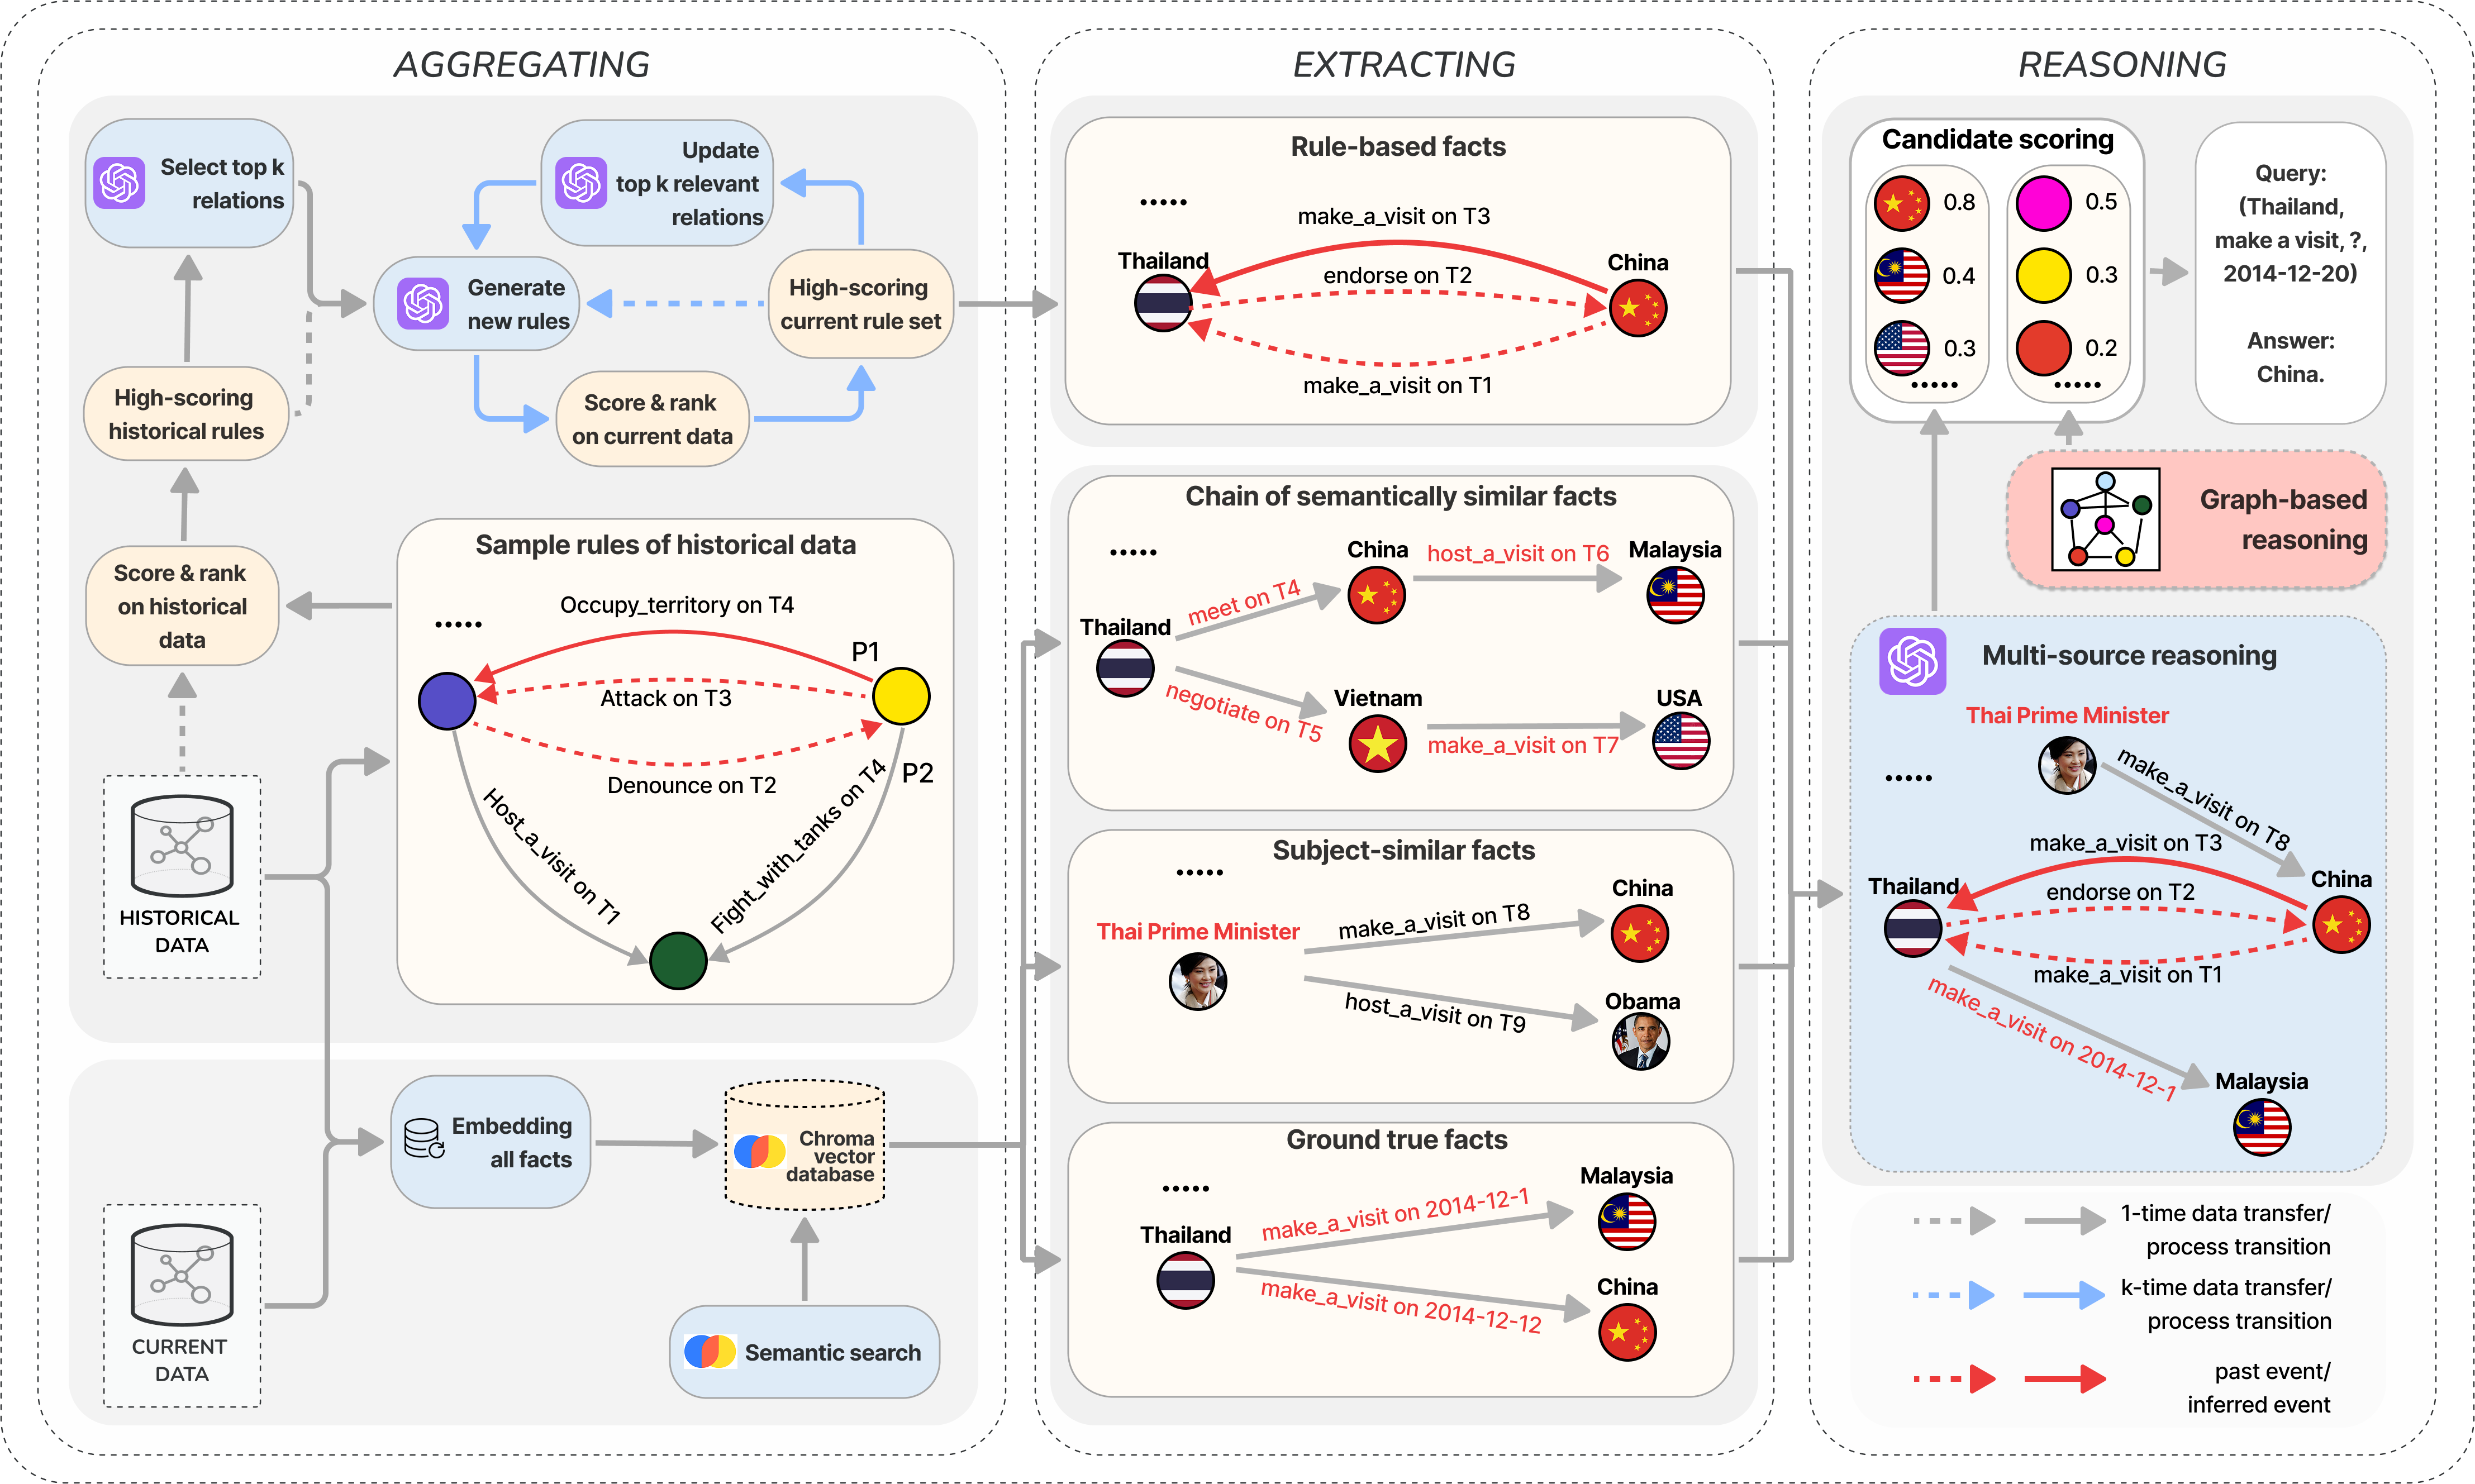
\includegraphics[width=15cm]{images/Framework01.png}
% \includesvg[width=\textwidth]{images/Framework01.svg}
\caption{MSKGen bắt đầu với hai quá trình song song: Trích xuất sự kiện dựa trên luật (Rule-based Facts Extraction) liên tục sử dụng LLMs để tạo luật từ các luật lịch sử được lấy mẫu, tinh chỉnh lặp đi lặp lại các luật mới dựa trên đánh giá từ dữ liệu hiện tại, và trích xuất các sự kiện chất lượng cao từ các luật đã tinh chỉnh; và Truy xuất sự kiện ngữ nghĩa (Semantic Facts Retrieval) nhúng các sự kiện vào cơ sở dữ liệu vector và truy xuất các sự kiện tương đồng ngữ nghĩa, sự kiện tương đồng chủ thể, và sự kiện chân lý nền sử dụng khái niệm RAG. Các sự kiện này được kết hợp trong Suy luận đa nguồn (Multi-Source Reasoning), nơi LLMs tổng hợp câu trả lời đặc thù cho truy vấn bằng cách tích hợp thông tin đa dạng và đồng bộ về mặt ngữ nghĩa.} 
\label{fig1}
\end{figure}

\section{Trích xuất sự kiện dựa trên luật}

\subsection{Trích xuất các luật lịch sử điểm cao và các quan hệ liên quan top k}

\paragraph{Lấy mẫu luật lịch sử.}
Giai đoạn đầu tiên của quá trình trích xuất sự kiện dựa trên luật (Rule-based Facts Extraction) bao gồm việc xác định các luật logic thời gian từ dữ liệu lịch sử bằng phương pháp duyệt ngẫu nhiên có thời gian (temporal random walk). Quá trình lấy mẫu tuân theo các bước chính sau. Đầu tiên, với một luật có độ dài \( l \), một chuỗi duyệt có độ dài \( l+1 \) được lấy mẫu, trong đó bước bổ sung tương ứng với phần đầu luật (rule head). Ở bước lấy mẫu đầu tiên \( m = 1 \), một cạnh \( (e_1, r_h, e_{l+1}, t_{l+1}) \) được lấy mẫu đồng nhất từ tất cả các cạnh có loại quan hệ \( r_h \). Bộ duyệt ngẫu nhiên thời gian sau đó lặp lại việc lấy mẫu các cạnh kề với đối tượng hiện tại cho đến khi thu được một chuỗi duyệt có độ dài \( l+1 \).

Để duy trì tính nhất quán thời gian, quá trình lấy mẫu sử dụng hàm xác suất chuyển tiếp (\ref{eq2}):
\begin{equation}
    \label{eq2}
    P(u; m, e_m, t_m) = \frac{\exp(t_u - t_m)}{\sum_{u' \in A(m, e_m, t_m)} \exp(t_{u'} - t_m)}
\end{equation}
nơi các cạnh gần thời gian hơn với nút hiện tại có xác suất lấy mẫu cao hơn. Điều này đảm bảo thứ tự thời gian được bảo toàn trong suốt quá trình duyệt và các sự kiện tương lai không thể ảnh hưởng đến sự kiện quá khứ. Cuối cùng, các chuỗi duyệt được lấy mẫu được chuyển đổi thành các luật bằng cách thay thế các thực thể thành biến số trong khi duy trì tham chiếu thực thể và bảo toàn các ràng buộc thời gian giữa các sự kiện.

\paragraph{Đánh giá chất lượng luật.}
Sau khi thu được các luật mẫu từ dữ liệu lịch sử thông qua duyệt ngẫu nhiên thời gian, chúng tôi triển khai quá trình trích xuất để xác thực chất lượng luật và tạo ra các quan hệ liên quan. Các luật mẫu trải qua quá trình đánh giá chất lượng sử dụng thước đo Kulczynski \cite{ref_article16} trên dữ liệu lịch sử, được định nghĩa (\ref{eq3}):
\begin{equation}
\label{eq3}
    Kulczynski(R) = \frac{1}{2} \left( \frac{r}{r_b} + \frac{r}{r_h} \right)
\end{equation}
trong đó: \( r_b \) biểu thị số cặp sự kiện thời gian thỏa mãn thân luật (rule body), \( r_h \) biểu thị số cặp sự kiện thời gian thỏa mãn đầu luật (rule head), \( r \) biểu thị số cặp sự kiện thỏa mãn cả điều kiện thân luật và đầu luật. Các luật vượt ngưỡng \( \gamma \) được phân loại là luật điểm cao.

\textit{Quá trình lựa chọn quan hệ.} Sau đánh giá chất lượng luật, với mỗi quan hệ trong dữ liệu hiện tại, chúng tôi triển khai quá trình lựa chọn quan hệ để xác định top-$k$ quan hệ liên quan nhất cho việc xây dựng luật thời gian. Quá trình này tận dụng Large Language Models (LLMs) thông qua phương pháp nhắc có cấu trúc. \textbf{User Message} chứa đầu vào biến đổi đặc thù cho từng truy vấn (đầu luật, các luật điểm cao, và các quan hệ khả dụng), trong khi \textbf{System Message} cung cấp hướng dẫn nhất quán xuyên suốt tất cả các trường hợp nhắc.


\begin{promptbox}{Prompt lựa chọn quan hệ liên quan}
\textbf{User Message:}
Cho trước một quan hệ đầu luật mục tiêu, hãy phân tích các luật điểm cao và các quan hệ khả dụng để xác định top-$k$ quan hệ liên quan nhất có thể tạo thành các luật thời gian có ý nghĩa.
\begin{itemize}
    \item \textbf{Đầu luật:} \texttt{\{rule\_head\}} - Quan hệ mục tiêu cho việc sinh luật
    \item \textbf{Tổ hợp logic hiện tại:} \texttt{\{high\_scoring\_rules\}} - Các luật điểm cao từ đánh giá luật
    \item \textbf{Quan hệ khả dụng:} \texttt{\{relation\_list\}} - Các quan hệ ứng viên để xây dựng luật
\end{itemize}

\textbf{System Message:} Chọn các quan hệ ứng viên thỏa mãn: Có liên kết ngữ nghĩa mạnh với quan hệ đầu luật, thể hiện khả năng dự đoán cao dựa trên các mẫu dữ liệu lịch sử và có thể tạo thành các luật thời gian có ý nghĩa khi kết hợp.
\end{promptbox}

\subsection{Sinh luật và tinh chỉnh lặp}

\paragraph{Sinh luật mới.}
Quá trình tạo các luật thời gian mới tận dụng Large Language Models (LLMs) thông qua phương pháp nhắc có cấu trúc. Cách tiếp cận này sử dụng các luật lịch sử điểm cao và các quan hệ liên quan top-k làm đầu vào. Chiến lược nhắc được thiết kế để hướng dẫn LLM tạo ra các luật logic thời gian toàn diện và có ý nghĩa....
\begin{promptbox}{Prompt sinh luật mới}
\textbf{User Message:}
Sinh các luật logic thời gian cho quan hệ mục tiêu thông qua Suy luận từng bước.
\begin{itemize}
    \item \textbf{Quan hệ mục tiêu:} \texttt{\{head\_relation\}(X, Y, T)} - Quan hệ mục tiêu cho việc sinh luật
    \item \textbf{Luật tham chiếu:} \texttt{\{high\_scoring\_rules\}} - Các luật tham chiếu điểm cao
    \item \textbf{Quan hệ ứng viên được cung cấp:} \texttt{\{relevant\_relations\}} - Các quan hệ ứng viên được cung cấp
\end{itemize}

\textbf{System Message:} Sử dụng các quan hệ từ phần thân của các luật tham chiếu và các quan hệ ứng viên được cung cấp, đảm bảo mỗi luật được sinh ra: duy trì tính nhất quán thời gian, tạo ra các liên kết ngữ nghĩa có ý nghĩa và hình thành các đường dẫn suy luận thời gian hợp lệ.\\
Ví dụ:

\begin{itemize}
    \item \textbf{Quan hệ mục tiêu:} Make a visit(X0, X1, T)
    \item \textbf{Luật tham chiếu:}
    \begin{itemize}
        \item Make a visit(X0, X1, T) $\leftarrow$ Host a visit(X1, X0, T0)
        \item Make a visit(X0, X2, T3) $\leftarrow$ Consult(X0, X1, T0)
    \end{itemize}
    \item \textbf{Quan hệ ứng viên được cung cấp:} Praise or endorse(X0, X1, T), Plan to meet(X0, X1, T), Engage in negotiation(X0, X1, T)
    $\Rightarrow$ \textbf{Luật sinh ra:} Make a visit(X0, X1, T3) $\leftarrow$ Endorse(X0, X1, T0) $\land$ Plan to meet(X1, X0, T1) $\land$ Host a visit(X0, X1, T2)
\end{itemize}
\end{promptbox}


\paragraph{Đánh giá và xếp hạng luật.}
Các luật được tạo ra trải qua đánh giá chất lượng sử dụng thước đo Kulczynski để so sánh chất lượng giữa các luật trong tập Generated rules dựa trên việc đánh giá chúng trên dữ liệu hiện tại. Thước đo Kulczynski, như đã định nghĩa trước đó, được sử dụng để đánh giá chất lượng luật. Các luật vượt ngưỡng $\gamma$ được thêm vào tập luật dưới dạng các luật hiện tại điểm cao. Quá trình đánh giá này đảm bảo chỉ các luật có độ chính xác và phạm vi bao phủ đủ tiêu chuẩn được giữ lại để sử dụng tiếp trong quá trình suy luận đồ thị tri thức thời gian.

\paragraph{Tinh chỉnh tập quan hệ liên quan: Cập nhật tập quan hệ liên quan Top k của mỗi đầu luật.}
Với mỗi đầu luật, chúng tôi đánh giá chất lượng quan hệ thông qua phép tính tỷ lệ (\ref{eq4}):
\begin{equation}
    \label{eq4}
    Quality(rel_i) = \frac{N_{high}(rel_i)}{N_{total}(rel_i)}
\end{equation}

trong đó $N_{high}(rel_i)$ biểu thị số lượng luật điểm cao chứa quan hệ $i$, và $N_{total}(rel_i)$ biểu thị tổng số luật được tạo ra chứa quan hệ $i$. Quá trình tinh chỉnh xác định $n$ quan hệ cuối (trong số $k$) dựa trên điểm chất lượng và cập nhật chúng thông qua lựa chọn có hướng dẫn bởi LLM:

\begin{promptbox}{Prompt tinh chỉnh tập quan hệ liên quan}
\textbf{User Message:}
Cho trước một đầu luật và các quan hệ hiệu suất thấp của nó, phân tích các luật điểm cao và các quan hệ khả dụng để xác định các quan hệ thay thế có thể nâng cao chất lượng luật thời gian.
\begin{itemize}
    \item \textbf{Đầu luật:} \texttt{\{rule\_head\}} - Quan hệ mục tiêu cho việc sinh luật
    \item \textbf{Tổ hợp logic hiện tại:} \texttt{\{high\_scoring\_rules\}} - Các luật điểm cao từ đánh giá luật
    \item \textbf{Quan hệ hiệu suất thấp:} \texttt{\{low\_quality\_relations\}} - Các quan hệ cần thay thế
    \item \textbf{Quan hệ khả dụng:} \texttt{\{relation\_list\}} - Các quan hệ ứng viên để thay thế
\end{itemize}

\textbf{System Message:} Lựa chọn các quan hệ thay thế có: Kết nối ngữ nghĩa mạnh với đầu luật và thể hiện khả năng dự đoán cao dựa trên các tổ hợp logic hiện tại.
\end{promptbox}

\paragraph{Cải tiến lặp.}
Toàn bộ quá trình hoạt động theo chu kỳ liên tục, nơi các luật mới được tạo ra bằng cách sử dụng các quan hệ đã cập nhật và các luật điểm cao mới, sau đó tiến hành đánh giá chất lượng và tinh chỉnh quan hệ. Quá trình này tiếp tục cho đến khi tập luật đạt được số lần lặp xác định trước, cuối cùng tạo ra tập luật hoàn thiện.

\subsection{Trích xuất sự kiện dựa trên luật}

\paragraph{Quá trình trích xuất sự kiện dựa trên luật.}
Với một truy vấn $q = (e_s, r, ?, t_q)$, chúng tôi lọc các luật từ tập luật hiện tại điểm cao nơi đầu luật khớp với $r$. Chúng tôi sau đó cụ thể hóa các luật này bằng cách thay thế thực thể truy vấn $e_s$ vào vị trí thích hợp, duy trì ràng buộc thời gian. Bằng cách tìm kiếm trong dữ liệu hiện tại các mẫu sự kiện phù hợp thỏa mãn thân luật $\bigwedge_{i=1}^{l-1} r_i(e_s, e_o, t_i)$, chúng tôi trích xuất các sự kiện dựa trên luật hoàn chỉnh tạo thành các chuỗi lý luận nhất quán thời gian để dự đoán các câu trả lời tiềm năng.

\vspace{1em}
\section{Trích xuất sự kiện theo ngữ nghĩa}

Phương pháp trích xuất sự kiện thứ hai mà MSKGen sử dụng là phương pháp trích xuất dựa theo ngữ nghĩa sử dụng ý tưởng của RAG để giải quyết bài toán suy luận trên đồ thị tri thức theo thời gian. Không giống các phương pháp truy xuất "khô cứng" mà chỉ phụ thuộc hoàn toàn vào việc làm khớp các lược đồ/từ khóa (schema matching) một cách chính xác, phương pháp này sử dụng các vector nhúng tiềm ẩn để nắm bắt sự tương đồng về ngữ nghĩa giữa các chủ thể, sự kiện. Điều này giúp mở rộng không gian tìm kiếm và cung cấp ngữ cảnh phong phú hơn cho mô hình ngữ ngôn lớn trong quá trình suy luận.

\vspace{1em}
\subsection{Tiền xử lý dữ liệu}
Để chuẩn bị cho giai đoạn truy xuất, MSKGen sẽ thực hiện tiền xử lý và nhúng tất cả các sự kiện (fact) vào một cơ sở dữ liệu chung gọi là cơ sở dữ liệu vector.

MSKGen bắt đầu bắt việc chuyển đổi tất cả các sự kiện từ định dạng văn bản có cấu trúc gồm bốn thành phần ($s, r, o, t$) thành một câu hoàn chỉnh diễn tả đầy đủ nội dung sự kiện được ngụ ý bởi bốn thành phần này. Ví dụ bộ bốn (\textit{Malaysia, make\_a\_visit, Thailand, 2014-9-12}) sẽ được chuyển thành một câu hoàn chỉnh \textit{Malaysia made a visit to Thailand on 2014-9-12}. Quy trình này đảm bảo thông tin ngữ nghĩa và bối cảnh của mỗi sự kiện sẽ được giữ nguyên khi nhúng sang không gian vector.

Để trích xuất tri thức ẩn chứa trong mỗi fact, MSKGen sử dụng kĩ thuật nhúng (embedding) để chuyển văn bản thành các vector đặc trưng. Trong quá trình này, \textbf{Chroma} được chọn làm cơ sở dữ liệu vector vì đây là một hệ thống lưu trữ chuyên dụng, được thiết kế cho việc lưu trữ và truy vấn các vector nhúng với hiệu suất cao. Bằng cách sử dụng tính năng tìm kiếm theo độ tương đồng cosine của Chroma, các sự kiện có nội dung tương đồng về ngữ nghĩa với sự kiện truy vấn có thể được truy xuất một cách chính xác ngay cả khi giữa chúng không có sự trùng khớp về từ khóa.

\vspace{1em}
\subsection{Xây dựng cơ sở dữ liệu vector}

Cơ sở dữ liệu trong MSKGen được thiết kế để không chỉ đơn giản là một hệ thống lưu trữ vector nâng cao mà còn cung cấp một cấu trúc lưu trữ tài liệu linh hoạt. Cụ thể, mỗi sự kiện sẽ được chuyển đổi thành một tài liệu (document) với ba thành phần chính:
\begin{itemize}
    \item \textbf{Metadata:} Thành phần này đóng vai trò như một bộ lọc (filter) trước khi quá trình tìm kiếm tài liệu được thực hiện. Metadata của mỗi tài liệu được thiết kế dưới dạng một từ điển (dictionary) $\mathcal{M} = \{\mathcal{S, R, E, T}\}$, trong đó $\mathcal{S, R, E, T}$ lần lượt là thực thể chủ ngữ, mối quan hệ giữa 2 thực thể trong sự kiện, thực thể vị ngữ và mốc thời gian. Cách thiết kế này giúp lọc ra các tài liệu khônng muốn, thu hẹp không gian tìm kiếm, đồng thời nâng cao cả độ chính xác lẫn tốc độ tìm kiếm.
    \item \textbf{Nội dung trang (page content):} Đây là chuỗi văn bản mô tả sự kiện có được sau giai đoạn tiền xử lý. Thành phần này sẽ được nhúng thành vector và vector đó sẽ được dùng để so sánh sự tương đồng với vector của truy vấn.
    \item \textbf{Vector nhúng (vector embedding):} Đây là vector số biểu diễn cho nội dung trang của tài liệu sau khi đã được nhúng. Việc chuyển đổi nội dung trang sang vector nhúng được thực hiện bởi mô hình nhúng được huấn luyện sẵn của OpenAI - \textbf{text-embedding-3-large} \cite{ref_article18}.
\end{itemize}

\vspace{1em}
\subsection{Phương pháp truy xuất ngữ nghĩa}

Với truy vấn $\mathcal{Q}$, MSKGen sẽ trích xuất ra ba thành phần - chủ thể $\mathcal{S}$, quan hệ $\mathcal{R}$ và mốc thời gian $\mathcal{T}$ - để hỗ trợ quá trình truy xuất. Để truy xuất các sự kiện mà chủ thể hoặc quan hệ của nó có ngữ nghĩa tương tự với $\mathcal{S, R}$ thông qua cơ sở dữ liệu vector. Đầu tiên, MSKGen sử dụng bộ lọc metadata để giảm không gian tìm kiếm. Sau khi đã loại bỏ bớt các tài liệu không cần thiết, MSKGen sẽ tiếp tục việc tìm kiếm trên các tài liệu còn lại. Cụ thể, tùy vào chiến lược truy xuất thì chủ thể $\mathcal{S}$ hoặc quan hệ $\mathcal{R}$ sẽ được nhúng thành vector truy vấn $\mathcal{Q}$ bằng cách sử dụng mô hình text-embedding-3-large (\ref{eq:query-embed}):
\begin{equation}  
\label{eq:query-embed}  
Q = \text{text-embedding-3-large}(\mathcal{R}). 
\end{equation}

Sau đó, MSKGen sẽ truy xuất top k tài liệu mà vector nhúng của nội dung trang có sự tương đồng về mặt ngữ nghĩa nhất với vector truy vấn $\mathcal{Q}$ dựa trên độ đo tương đồng cosine (\ref{eq:cos-sim_1},\ref{eq:top-sim_2}):
\begin{equation}  
\label{eq:cos-sim_1}  
\text{Cos-Sim}(Q, d_{i})   
\,=\, \frac{Q \cdot d_{i}}{\|Q\|\;\|d_{i}\|}  
\end{equation}

\begin{equation}  
\label{eq:top-sim_2}  
\text{Top-}k   
= \arg\max_{d_i \in D}^{k}\,\text{Cos-Sim}(Q, d_i).    
\end{equation} 

Trong đó $\cdot$ là phép nhân vô hướng, $\|\cdot\|$ biểu diễn chuẩn (norm) của vector, $d_{i}$ kí hiệu vector nhúng của tài liệu thứ $i$ và $\text{Top-}k$ là tập hợp $k$ tài liệu mà nội dung trang của chúng có sự tương đồng về mặt ngữ nghĩa với truy vấn nhất.

\vspace{1em}
\subsection{Chiến lược truy xuất sự kiện}

Dự đoán của các mô hình ngôn ngữ lớn phụ thuộc rất nhiều vào ngữ cảnh được cung cấp. Việc chỉ truy xuất các sự kiện khớp cứng với từ khóa cho trước (ICL) hoặc các sự kiện dạng chuỗi lịch sử (CoH) sẽ bỏ qua những kết nối ngữ nghĩa quan trọng. Chẳng hạn, các quyết định hợp tác của Malaysia có thể chịu ảnh hưởng không chỉ bởi các đối tác trước đây mà còn bởi các sự kiện khác như việc viếng thăm hoặc những cuộc họp quan trọng. Vì vậy đối với một truy vấn dạng bộ bốn $\mathcal{Q = (S, R, ?, T})$, MSKGen thực hiện chiến lược truy xuất cho ba tập hợp sự kiện sau:
\begin{itemize}
    \item \textbf{Chuỗi các sự kiện tương đồng về mặt ngữ nghĩa:} Đây là một chuỗi các sự kiện bắt đầu từ chủ thể $\mathcal{S}$ và có quan hệ tương đồng về mặt ngữ nghĩa với quan hệ $\mathcal{R}$. Các chuỗi sự kiện này sẽ được lưu vào một tập hợp, kí hiệu là $H_C$. Tập $H_C$ sẽ giúp LLM thực hiện suy luận đa bước (multi-hop reasoning), do đó các sự kiện trong $H_C$ sẽ được sắp xếp theo thứ tự tăng dần của thời gian.
    \item \textbf{Các sự kiện có chủ thể tương đồng với chủ thể truy vấn:} Một hạn chế lớn thường bị bỏ qua là khi chủ thể $\mathcal{S}$ trong truy vấn hoàn toàn mới và không có dữ liệu lịch sử, khiến LLM thiếu thông tin để suy luận. Để khắc phục điều này, MSKGen thay thế $\mathcal{S}$ bằng các thực thể tương tự có các mối quan hệ liên quan. Nếu không có sự kiện lịch sử nào liên quan tới $\mathcal{S}$, LLM sẽ sử dụng các sự kiện từ các thực thể tương tự này vì chúng thường chia sẻ những hình hành vi chung. Các sự kiện này được lưu trong tập $H_S$ và sẽ được dùng để bổ sung ngữ cảnh cho LLM, đặc biệt khi tập $H_C$ không đủ hoặc bị thiếu.
    \item \textbf{Ground true của những sự kiện tương tự vừa xảy ra trước truy vấn $\mathcal{Q}$:} Để tránh việc LLM liên tục trả lời sai đối với các truy vấn cùng chủ thể $\mathcal{S}$ và quan hệ $\mathcal{R}$ và có mốc thời gian gần nhau, MSKGen sẽ cung cấp thêm cho LLM các ground true của những sự kiện tương tự vừa xảy ra trước sự kiện truy vấn $\mathcal{Q}$. Những sự kiện này sẽ được lưu vào tập $H_G$.
\end{itemize}

Việc lưu trữ các sự kiện được truy xuất vào 3 tập khác nhau $H_C, H_S$ và $H_G$ là không khả thi vì sẽ tiêu tốn quá nhiều token đầu vào dẫn đến có thể vượt quá độ dài ngữ cảnh mà mô hình ngôn ngữ lớn cho phép. Do đó, MSKGen giới hạn các tập này chỉ còn các sự kiện phù hợp nhất, cụ thể là các sự kiện lịch sử từ quá khứ xa và gần. Chiến lược lựa chọn này giúp duy trì các mối liên hệ lâu dài và ngắn hạn quan trọng, qua đó nâng cao độ chính xác dự đoán của LLM. 

\vspace{1em}
\section{Suy luận tri thức đa nguồn}
Đối với các truy vấn theo thời gian có dạng $\mathcal{Q = (S, R, ?, T)}$, MSKGen sẽ cung cấp các sự kiện truy xuất dựa trên luật và các sự kiện truy xuất dựa trên ngữ nghĩa cho LLM thông qua User Message và System Message.

System Message chứa một hướng dẫn chi tiết, điều phối quá trình suy luận qua các giai đoạn thao tác rời rạc. Mỗi giai đoạn kết hợp các chỉ dẫn theo ngữ cảnh với ví dụ minh họa cho từng nhóm sự kiện, giúp mô hình tổng hợp dần dần các bằng chứng thời gian trong khi vẫn duy trì mạch suy luận nhất quán. Tất cả các sự kiện được cung cấp cho LLM sẽ được gửi thông qua User Message.

MSKGen giới hạn LLM chỉ trả về $k$ ứng viên có khả năng cao nhất, nhờ vậy giảm bớt việc lãng phí token cho các kết quả kém khả thi. Cuối cùng, MSKGen hợp nhất hai danh sách ứng viên — một từ suy luận dựa trên các sự kiện truy xuất từ luật và một từ suy luận dựa trên các sự kiện truy xuất dựa trên ngữ nghĩa — thành một danh sách ứng viên cuối cùng duy nhất.

\vspace{1em}
\section{Cách tính điểm các ứng viên}

Điểm số cuối cùng của MSKGen trả về bao gồm 2 thành phần chính: điểm số của LLM (LLM-based score) và điểm số lấy từ mô hình đồ thị đã được huấn luyện sẵn (Graph-based score).

\vspace{1em}
\subsection{Điểm số dự đoán của LLM}

Với mỗi thực thể ứng cử viên $c_i$ từ tập ứng cử viên $C$ trả về bởi LLM cho truy vấn $\mathcal{Q}$, MSKGen sẽ tính điểm nó bằng cách kết hợp thứ hạng (rank) của thực thể này được xếp bởi LLM và độ chênh lệch thời gian giữa mốc thời gian $\mathcal{T}$ của truy vấn với mốc thời gian gần nhất mà $c_i$ tương tác với $\mathcal{S}$ (được kí hiệu là $\mathcal{T}_{c_i}$) (\ref{eq:score-llm}):
\begin{equation}  
\label{eq:score-llm}  
\text{score}^{c_i}_{\text{LLM}}   
= \alpha \times \Bigl(1 - \frac{r_{c_i}}{k}\Bigr)  
\;+\; (1 - \alpha)\,\times\, e^{\lambda \,\bigl(\mathcal{T}_{c_i} - \mathcal{T}\bigr)}   
\end{equation}

Trong đó, $\lambda$ biểu thị cho hệ số suy giảm theo thời gian (time decay), $k$ là số lượng ứng cử viên tối đa được LLM trả về và $\alpha$ là trọng số cho dự đoán của LLM. Đối với các thực thể nằm trong tập thực thể của bộ dữ liệu nhưng không có trong dự đoán của LLM thì điểm số của chúng sẽ là 0.

\vspace{1em}
\subsection{Điểm số từ dự đoán của mô hình học sâu theo phương pháp nhúng đồ thị}

Do hạn chế về đầu ra, danh sách ứng viên được tạo ra bởi LLM có thể không có khả năng để khớp với đáp án của toàn bộ câu truy vấn. Để nâng cao độ chính xác của kết quả cuối cùng, MSKGen có tích hợp thêm kết quả của mô hình học sâu theo phương pháp nhúng đồ thị. Điểm số của ứng cử viên $c_i$ có từ mô hình học sâu theo phương pháp nhúng kí hiệu là $\text{score}_G^{c_i}$.

\vspace{1em}
\subsection{Điểm số cuối cùng}

Điểm số cuối cùng của một thực thể ứng cử viên sẽ là sự tổng hợp từ hai điểm số trên (\ref{eq:final-score}):
\begin{equation}
    \label{eq:final-score}
    \text{score}^{c_i} = \alpha \times \text{score}^{c_i}_{\text{LLM}} + (1 - \alpha) \times \text{score}_G^{c_i}
\end{equation}

Trong đó $\alpha$ và $1 - \alpha$ lần lượt kí hiệu cho trọng số dự đoán của LLM và trọng số dự đoán của mô hình học sâu theo phương pháp nhúng.



\chapter{Kết quả thí nghiệm}
\label{Chapter5}
Chương này sẽ bắt đầu bằng việc giới thiệu chi tiết về các tập dữ liệu
chuẩn được sử dụng trong quá trình thí nghiệm. Tiếp theo, khóa luận sẽ
trình bày các độ đo được sử dụng để đánh giá hiệu quả của mô hình dự
đoán liên kết đã được đề xuất. Để so sánh hiệu quả của mô hình được
đề xuất với các phương pháp đã có, khóa luận tiếp tục tóm tắt những mô
hình cơ sở được lựa chọn. Sau đó, khóa luận sẽ tiến hành các thí nghiệm liên quan để so sánh hiệu suất của mô hình được đề xuất với các mô hình cơ sở này. Quá trình so sánh này sẽ giúp đánh giá hiệu quả của mô hình MSKGen trong bối cảnh chung của nghiên cứu suy luận trên đồ thị tri thức thời gian.

\section{Bộ dữ liệu}
Khóa luận này tập trung vào việc đánh giá hiệu quả của các mô hình suy luận trên đồ thị tri thức thời gian ở 3 tập dữ liệu: ICEWS14, GDELT và YAGO. 

ICEWS14, được trích xuất từ bộ dữ liệu ICEWS (Integrated Crisis Early Warning System), là tập các thông tin liên quan đến vấn đề chính trị. Nó tập chung vào các mối quan hệ giữa các thực thể như thủ tướng, người hoặc nhóm người, các quốc gia, tổ chức chính trị... Các mối quan hệ này được cập nhật hằng ngày, liên quan đến những hành động cụ thể. Các nghiên cứu trước đây đã sử dụng ICEWS nói chung và ICEWS14 nói riêng cho các tác vụ dưới dòng trong lĩnh vực khai thác dữ liệu đồ thị, tiêu biểu là dự đoán liên kết. Là một tập con của tập ICEWS, ICEWS14, như tên của nó, chỉ tập trung vào các sự kiện xảy ra vào năm 2014.

YAGO là một cơ sở dữ liệu lớn kết hợp WordNet (cơ sở dữ liệu về từ vựng) và thông tin từ Wikipedia. YAGO miêu tả đa dạng các thực thể
trong thế giới thực và các mối quan hệ giữa chúng. Cấu trúc của bộ dữ liệu này có hơi khác biệt khi thay vì cung cấp các thông tin thời gian như trong bộ bốn, các thông tin thời gian của YAGO được biểu diễn bằng 2 thông tin riêng biệt: bắt đầu lúc (occurFrom) và kết thúc lúc (occurUntil). Vì thế, các dữ liệu trong tập này thường được biểu diễn dưới dạng bộ năm và điều này đòi hỏi các bước tiền xử lí dữ liệu để có thể ánh xạ bộ dữ liệu này về định dạng các bộ tứ.

 GDELT được chiết xuất từ tập GDELT (Global Database of Events, Language, and Tone) và cả hai tập này dù giống tên nhưng không hề giống nhau. Khi sử dụng trong lĩnh vực khai thác dữ liệu đồ thị GDEL sẽ tự được hiểu là một tập con của tập GDELT lớn hơn. Tập GDELT lớn thực chất là tên của một dự án dữ liệu mở nhằm theo dõi và thu thập hành vi của con người qua các nền tảng truyền thông. Nó bao gồm thông tin của sự kiện, những cảm xúc, vị trí hay những người có liên quan đến sự kiện đó. Bộ dữ liệu đã có những dữ liệu đầu tiên vào năm 1979 và được cập nhật thường xuyên cho đến hiện tại.

 Chi tiết của từng bộ dữ liệu sẽ được mô tả ở 2 bảng~\ref{tab:table51} và~\ref{tab:table52}:

\begin{table}[H]
\caption{Thông số huấn luyện, kiểm thử và xác thực của ba bộ dữ liệu
 tiêu chuẩn}
\label{tab:table51}
\begin{adjustbox}{width=\textwidth}
\begin{tabular}{|l|l|l|l|}
\hline
Tập dữ  liệu & Kích thước tập train & Kích thước tập valid & Kích thước tập test \\ \hline
ICEWS14      & 74854                & 8514                 & 7371                \\ \hline
GDELT        & 79319                & 9957                 & 9715                \\ \hline
YAGO         & 220393               & 28948                & 22765               \\ \hline
\end{tabular}
\end{adjustbox} 
\end{table}

\begin{table}[H]
\caption{Thông số về cấu trúc của ba bộ dữ liệu tiêu chuẩn}
\label{tab:table52}
\begin{adjustbox}{width=\textwidth}
\begin{tabular}{|l|l|l|l|}
\hline
Tập dữ  liệu & Số lượng thực thể & Số lượng quan hệ & Chênh lệch thời gian \\ \hline
ICEWS14      & 7128              & 230              & 1 ngày               \\ \hline
GDELT        & 5850              & 238              & 15 phút              \\ \hline
YAGO         & 10778             & 23               & 1 năm                \\ \hline
\end{tabular}
\end{adjustbox} 
\end{table}

\section{Độ đo đánh giá}
Để đánh giá độ hiệu quả của MSKGen trong khả năng suy luận trên đồ thị tri thức theo thời gian, chúng tôi sẽ áp dụng một số độ đo tiêu chuẩn cho lĩnh vực dự đoán liên kết trong đồ thị tri thức thời gian. Những độ đo này cung cấp cái nhìn sâu sắc về hiệu suất của mô hình, bao gồm độ chính xác và khả năng dự đoán. Hơn nữa, chúng là nền tảng để so sánh và chứng minh hiệu quả của MSKGen so với các mô hình khác. Hai độ đo chính được sử dụng là Mean Reciprocal Rank (MRR) và Hits@k.

Mean Rank (MR) phản ánh thứ hạng trung bình của các bộ tứ được dự đoán. MR càng cao, mô hình càng có khả năng dự đoán chính xác. Tuy
nhiên, một bộ tứ có điểm thấp bị ảnh hưởng quá lớn đến giá trị của MR. Để khắc phục hạn chế này, MRR được sử dụng. MRR ưu tiên những lần 
dự đoán có kết quả tốt bằng cách lấy giá trị nghịch đảo của điểm xếp hạng. Điều này giúp giảm thiểu ảnh hưởng tiêu cực của những lần dự đoán kém 
chính xác, tăng cường sự phản ánh hiệu quả chung của mô hình.
\begin{equation}
    \label{eq:MRR}
    MRR = \frac{1}{|p|} \sum_{r \in p} r^{-1}
\end{equation}

Hits@k cung cấp thông tin về khả năng đoán đúng của mô hình trong phạm vị k kết quả cao nhất. Ví dụ, Hits@10 là xác suất có xuất hiện kết quả đúng trong 10 phần tử có điểm xếp hạng cao nhất của mô hình. Độ đo này không quan tâm tới vị trí chính xác của đáp án mà chỉ quan tâm là nó có nằm trong k phần tử đầu tiên hay không mà thôi. Giá trị Hits@k càng cao thì khả năng dự đoán của mô hình càng cao. Giá trị của k thường được sử dụng là 1, 3 và 10 để biểu diễn khả năng dự đoán ở các giới hạn tương ứng.
\begin{equation}
    \label{eq:hit@k}
    Hits@k = \frac{1}{|p|} \sum_{r \in p} (1 \text{ if } r \leq k \text{ else } 0)
    \tag{x}
\end{equation}

\section{Thiết lập đánh giá}

Theo bài báo ..., có hai thiết lập đánh giá:
\begin{itemize}
    \item \textbf{Thiết lập thô (Raw)}: Thiết lập này sẽ đơn giản là truy xuất thứ hạng của các thực thể ứng viên đã được sắp xếp theo điểm số
    dự đoán và từ đó tính toán độ đo đánh giá dựa theo thứ hạng của thực thể chính xác cho câu truy vấn. 
    \item \textbf{Thiết lập bộ lọc nhận thức thời gian (Time-aware filter)}: Thiết lập này cũng sẽ truy xuất điểm số của các thực thể ứng viên đã được sắp xếp 
    và loại bỏ các dự đoán hợp lệ nhưng không chính xác với câu truy vấn hiện tại trước khi xếp hạng, giúp ngăn chặn việc có nhiều hơn một thực thể chính xác cho một câu truy vấn.
    Ví dụ, với truy vấn \textit{(Malaysia, Make\_visit, ?, 2014-1-12)} và đáp án đúng là \textit{Thailand}, các dự đoán hợp lệ khác như 
    \textit{China} hay \textit{Vietnam} sẽ bị loại bỏ để đảm bảo rằng chỉ có một thực thể chính xác duy nhất được xếp hạng.
\end{itemize}

Trong khóa luận này, chúng tôi sẽ sử dụng thiết lập bộ lọc nhận thức thời gian để đánh giá mô hình MSKGen. Thiết lập này giúp đảm bảo rằng các dự đoán được đánh giá là chính xác và phù hợp với ngữ cảnh thời gian của câu truy vấn, từ đó cung cấp cái nhìn rõ ràng hơn về hiệu suất của mô hình trong việc suy luận trên đồ thị tri thức thời gian.
\section{Các mô hình cơ sở}
Để đánh giá hiệu quả của mô hình FTPComplEx, chúng tôi tiến hành so sánh một cách khách quan với 3 nhóm mô hình: nhóm mô hình học sâu được huấn luyện trên đồ thị, nhóm mô hình suy luận dựa trên luật và nhóm mô hình suy luận nhờ LLM. Việc lựa chọn các mô hình đối chiếu này được thực hiện dựa trên sự đa dạng về kỹ thuật và cách tiếp cận, giúp việc so sánh với MSKGen trở nên đầy thuyết phục hơn. 

Nhóm mô hình học sâu được huấn luyện trên đồ thị bao gồm:
\begin{itemize}
    \item \textbf{RE-NET}
    \item \textbf{RE-GCN}
    \item \textbf{TiRGN}
    \item \textbf{HGLS}
\end{itemize}

Nhóm mô hình suy luận dựa trên luật bao gồm:
\begin{itemize}
    \item \textbf{TLogic}
\end{itemize}

Nhóm mô hình suy luận nhờ LLM bao gồm:
\begin{itemize}
    \item \textbf{GPT-Neox-ICL}
    \item \textbf{TiRGN-CoH}
    \item \textbf{GenTKG}
\end{itemize}

\section{Cài đặt siêu tham số thực nghiệm}
Các thực nghiệm được thực hiện trên NVIDIA GeForce RTX 3070 8GB VRAM. MSKGen được chạy thực nghiệm nhiều lần để tìm ra các siêu tham số
tốt nhất của từng giai đoạn ở mỗi tập dữ liệu:
\begin{itemize}
    \item Trong giai đoạn trích xuất sự kiện dựa theo luật, số lượng vòng lặp để cập nhật luật được thực hiện là 5, 
ngưỡng điểm để lọc ra các luật có chất lượng cao là $\gamma = 0.15$ trên cả ba tập dữ liệu.
    \item Trong giai đoạn trích xuất sự kiện theo ngữ nghĩa, MSKGen sử dụng mô hình \textbf{GPT-4o-mini} cho việc suy luận. 
    Hệ số suy giảm theo thời gian $\lambda$, trọng số của xếp hạng các thực thể ứng viên được dự đoán bởi LLM $\alpha$ và
    số lượng ứng cử viên tối đa mà LLM có thể trả về $k$ lần lượt là 0.1, 0.5 và 10 trên cả ba tập dữ liệu. 
    \item Ở bước tổng hợp kết quả dự đoán cuối cùng, \textbf{TiRGN} là mô hình được chọn để lấy điểm số từ dự đoán của mô hình học sâu 
    huấn luyện trên đồ thị $score_{G}^{c_i}$. Trọng số cho điểm số từ dự đoán của LLM $\alpha$ và của TiRGN $1 - \alpha$
    trong điểm số cuối cùng trên từng tập dữ liệu được thể hiện trong bảng~\ref{tab:table53}:
\end{itemize}

\begin{table}[H]
\caption{Trọng số của mỗi điểm số thành phần trong điểm số cuối cùng trên từng tập dữ liệu}
\label{tab:table53}
\begin{adjustbox}{width=\textwidth}
\begin{tabular}{|l|l|l|l|}
\hline
           & ICEWS14 & GDELT & YAGO \\ \hline
$\alpha$   & 0.6     & 0.6   & 0.85 \\ \hline
$1-\alpha$ & 0.4     & 0.4   & 0.15 \\ \hline
\end{tabular}
\end{adjustbox}  
\end{table}
  

\section{Kết quả thí nghiệm}
\subsection{Kết quả chính}

Bảng ~\ref{tab:table54},~\ref{tab:table55} và~\ref{tab:table56} trình bày kết quả thực nghiệm chính của MSKGen và 
các mô hình cơ sở khác trong việc suy luận trên đồ thị tri thức thời gian trên ba tập dữ liệu tiêu chuẩn bao gồm 
ICEWS14, GDELT và YAGO.

\begin{table}
\caption{Kết quả thực nghiệm của MSKGen và các mô hình khác trên tập dữ liệu ICEWS14 với thiết lập bộ lọc nhận thức thời gian. 
Điểm số cao nhất được \textbf{bôi đen} và điểm số tốt thứ hai được \underline{gạch chân}.}
\label{tab:table54}
\begin{adjustbox}{width=\textwidth}
% \begin{tabular}{|cc|ccc|ccc|ccc|}
% \hline
% \multicolumn{1}{|c|}{\multirow{2}{*}{Method}}      & \multirow{2}{*}{Model} & \multicolumn{3}{c|}{ICEWS14}                                             & \multicolumn{3}{c|}{GDELT}                                               & \multicolumn{3}{c|}{YAGO}                                                \\ \cline{3-11} 
% \multicolumn{1}{|c|}{}                             &                        & \multicolumn{1}{c|}{Hit@1} & \multicolumn{1}{c|}{Hit@3} & Hit@10         & \multicolumn{1}{c|}{Hit@1} & \multicolumn{1}{c|}{Hit@3} & Hit@10         & \multicolumn{1}{c|}{Hit@1} & \multicolumn{1}{c|}{Hit@3} & Hit@10         \\ \hline
% \multicolumn{1}{|c|}{\multirow{5}{*}{Graph-based}} & RE-NET~\cite{ref_article12}                 & 0.301                      & 0.440                      & 0.582          & 0.081                      & 0.158                      & 0.261          & 0.404                      & 0.530                      & 0.629          \\ \cline{2-2}
% \multicolumn{1}{|c|}{}                             & RE-GCN~\cite{ref_article13}                 & 0.313                      & 0.470                      & 0.613          & 0.084                      & 0.171                      & 0.299          & 0.468                      & 0.607                      & 0.729          \\ \cline{2-2}
% \multicolumn{1}{|c|}{}                             & TiRGN~\cite{ref_article22}                  & 0.338                      & {\ul 0.497}                & 0.650          & 0.136                      & {\ul 0.233}             & {\ul 0.376}    & {\ul 0.843}             & {\ul 0.913}             & {\ul 0.929}    \\ \cline{2-2}
% \multicolumn{1}{|c|}{}                             & HGLS~\cite{ref_article14}                   & 0.350                      & 0.490                      & {\ul 0.704}    & 0.118                      & 0.217                      & 0.332          & 0.806                      & 0.901                      & 0.919          \\ \hline
% \multicolumn{1}{|c|}{Rule-based}                   & TLogic~\cite{ref_article23}                 & 0.326                      & 0.483                      & 0.612          & 0.113                      & 0.212                      & 0.351          & 0.740                      & 0.789                      & 0.791          \\ \hline
% \multicolumn{1}{|c|}{\multirow{3}{*}{LLM-based}}   & GPT-Neox-ICL~\cite{ref_article08}           & 0.295                      & 0.406                      & 0.475          & 0.068                      & 0.120                      & 0.211          & 0.720                      & 0.810                      & 0.846          \\ \cline{2-2}
% \multicolumn{1}{|c|}{}                             & TiRGN-CoH~\cite{ref_article09}              & 0.330                      & 0.496                      & 0.649          & -                          & -                          & -              & -                          & -                          & -              \\ \cline{2-2}
% \multicolumn{1}{|c|}{}                             & GenTKG~\cite{ref_article10}                 & {\ul 0.363}                & 0.473                      & 0.528          & {\ul 0.134}                & 0.220                      & 0.300          & 0.792                      & 0.830                      & 0.843          \\ \hline
% \multicolumn{2}{|c|}{MSKGen (TiRGN)}                                        & \textbf{0.384}             & \textbf{0.525}             & \textbf{0.710} & \textbf{0.145}             & \textbf{0.235}                & \textbf{0.402} & \textbf{0.856}                & \textbf{0.929}                & \textbf{0.947} \\ \hline
% \end{tabular}
\begin{tabular}{|cc|cccc|}
\hline
\multicolumn{1}{|c|}{\multirow{2}{*}{Phương pháp}}     & \multirow{2}{*}{Mô hình} & \multicolumn{4}{c|}{ICEWS14}                                                                        \\ \cline{3-6} 
\multicolumn{1}{|c|}{}                                 &                          & \multicolumn{1}{c|}{MRR} & \multicolumn{1}{c|}{Hit@1} & \multicolumn{1}{c|}{Hit@3} & Hit@10         \\ \hline
\multicolumn{1}{|c|}{\multirow{4}{*}{Dựa trên đồ thị}} & RE-NET                   & 0.457                    & 0.301                      & 0.440                      & 0.582          \\ \cline{2-2}
\multicolumn{1}{|c|}{}                                 & RE-GCN                   & 0.415                    & 0.313                      & 0.470                      & 0.613          \\ \cline{2-2}
\multicolumn{1}{|c|}{}                                 & TiRGN                    & 0.440                    & 0.338                      & {\ul 0.497}                & 0.650          \\ \cline{2-2}
\multicolumn{1}{|c|}{}                                 & HGLS                     & {\ul 0.470}              & 0.350                      & 0.490                      & {\ul 0.704}    \\ \hline
\multicolumn{1}{|c|}{Dựa trên luật}                    & TLogic                   & 0.430                    & 0.326                      & 0.483                      & 0.612          \\ \hline
\multicolumn{1}{|c|}{\multirow{3}{*}{Dựa trên LLM}}    & GPT-Neox-ICL             & 0.322                    & 0.295                      & 0.406                      & 0.475          \\ \cline{2-2}
\multicolumn{1}{|c|}{}                                 & TiRGN-CoH                & 0.439                    & 0.330                      & 0.496                      & 0.649          \\ \cline{2-2}
\multicolumn{1}{|c|}{}                                 & GenTKG                   & -                        & {\ul 0.368}                & 0.479                      & 0.535          \\ \hline
\multicolumn{2}{|c|}{MSKGen}                                                      & \textbf{0.481}           & \textbf{0.384}             & \textbf{0.525}             & \textbf{0.710} \\ \hline
\end{tabular}
\end{adjustbox}  
\end{table}
\vspace{-5mm}

Trên tập dữ liệu ICEWS14 và GDELT, MSKGen đều đạt được kết quả tốt nhất (state-of-the-art) trong tất cả độ đo 
đánh giá, bao gồm 

\begin{table}
\caption{Kết quả thực nghiệm của MSKGen và các mô hình khác trên tập dữ liệu GDELT với thiết lập bộ lọc nhận thức thời gian. 
Điểm số cao nhất được \textbf{bôi đen} và điểm số tốt thứ hai được \underline{gạch chân}.}
\label{tab:table55}
\begin{adjustbox}{width=\textwidth}
\begin{tabular}{|cc|cccc|}
\hline
\multicolumn{1}{|c|}{\multirow{2}{*}{Phương pháp}}     & \multirow{2}{*}{Mô hình} & \multicolumn{4}{c|}{GDELT}                                                                          \\ \cline{3-6} 
\multicolumn{1}{|c|}{}                                 &                          & \multicolumn{1}{c|}{MRR} & \multicolumn{1}{c|}{Hit@1} & \multicolumn{1}{c|}{Hit@3} & Hit@10         \\ \hline
\multicolumn{1}{|c|}{\multirow{4}{*}{Dựa trên đồ thị}} & RE-NET                   & 0.105                    & 0.081                      & 0.158                      & 0.261          \\ \cline{2-2}
\multicolumn{1}{|c|}{}                                 & RE-GCN                   & 0.146                    & 0.084                      & 0.171                      & 0.299          \\ \cline{2-2}
\multicolumn{1}{|c|}{}                                 & TiRGN                    & {\ul 0.216}              & {\ul 0.136}                & {\ul 0.233}                & {\ul 0.376}    \\ \cline{2-2}
\multicolumn{1}{|c|}{}                                 & HGLS                     & 0.190                    & 0.118                      & 0.217                      & 0.332          \\ \hline
\multicolumn{1}{|c|}{Dựa trên luật}                    & TLogic                   & 0.175                    & 0.113                      & 0.212                      & 0.351          \\ \hline
\multicolumn{1}{|c|}{\multirow{3}{*}{Dựa trên LLM}}    & GPT-Neox-ICL             & 0.103                    & 0.068                      & 0.120                      & 0.211          \\ \cline{2-2}
\multicolumn{1}{|c|}{}                                 & TiRGN-CoH                & -                        & -                          & -                          & -              \\ \cline{2-2}
\multicolumn{1}{|c|}{}                                 & GenTKG                   & -                        & 0.134                      & 0.220                      & 0.300          \\ \hline
\multicolumn{2}{|c|}{MSKGen}                                                      & \textbf{0.218}           & \textbf{0.145}             & \textbf{0.235}             & \textbf{0.402} \\ \hline
\end{tabular}
\end{adjustbox}  
\end{table}
\vspace{-5mm}

\begin{table}
\caption{Kết quả thực nghiệm của MSKGen và các mô hình khác trên tập dữ liệu YAGO với thiết lập bộ lọc nhận thức thời gian. 
Điểm số cao nhất được \textbf{bôi đen} và điểm số tốt thứ hai được \underline{gạch chân}.}
\label{tab:table56}
\begin{adjustbox}{width=\textwidth}
\begin{tabular}{|cc|cccc|}
\hline
\multicolumn{1}{|c|}{\multirow{2}{*}{Phương pháp}}     & \multirow{2}{*}{Mô hình} & \multicolumn{4}{c|}{YAGO}                                                                           \\ \cline{3-6} 
\multicolumn{1}{|c|}{}                                 &                          & \multicolumn{1}{c|}{MRR} & \multicolumn{1}{c|}{Hit@1} & \multicolumn{1}{c|}{Hit@3} & Hit@10         \\ \hline
\multicolumn{1}{|c|}{\multirow{4}{*}{Dựa trên đồ thị}} & RE-NET                   & 0.478                    & 0.404                      & 0.530                      & 0.629          \\ \cline{2-2}
\multicolumn{1}{|c|}{}                                 & RE-GCN                   & 0.558                    & 0.468                      & 0.607                      & 0.729          \\ \cline{2-2}
\multicolumn{1}{|c|}{}                                 & TiRGN                    & {\ul 0.879}              & {\ul 0.843}                & {\ul 0.913}                & {\ul 0.929}    \\ \cline{2-2}
\multicolumn{1}{|c|}{}                                 & HGLS                     & 0.817                    & 0.806                      & 0.901                      & 0.919          \\ \hline
\multicolumn{1}{|c|}{Dựa trên luật}                    & TLogic                   & 0.767                    & 0.740                      & 0.789                      & 0.791          \\ \hline
\multicolumn{1}{|c|}{\multirow{3}{*}{Dựa trên LLM}}    & GPT-Neox-ICL             & 0.783                    & 0.720                      & 0.810                      & 0.846          \\ \cline{2-2}
\multicolumn{1}{|c|}{}                                 & TiRGN-CoH                & -                        & -                          & -                          & -              \\ \cline{2-2}
\multicolumn{1}{|c|}{}                                 & GenTKG                   & 0.804                    & 0.792                      & 0.830                      & 0.843          \\ \hline
\multicolumn{2}{|c|}{MSKGen}                                                      & \textbf{0.902}           & \textbf{0.856}             & \textbf{0.929}             & \textbf{0.947} \\ \hline
\end{tabular}
\end{adjustbox}  
\end{table}
\vspace{-5mm}

\subsection{Nghiên cứu loại bỏ}

\subsection{Một số nghiên cứu khác}

\chapter{KẾT LUẬN}
\label{Chapter6}

Chương này trình bày những kết quả nghiên cứu đạt được, những đóng góp mới, chỉ ra những hạn chế và thách thức còn tồn đọng, từ đó đưa ra những đề xuất, kiến nghị cho các hướng nghiên cứu tiếp theo, nhằm mở rộng và ứng dụng hiệu quả hơn các kết quả nghiên cứu trong thực tế.

\section{Kết luận chung}
Trong nghiên cứu này, chúng tôi đã giới thiệu MSKGen - một phương pháp tiếp cận mới cho bài toán suy luận đồ thị tri thức thời gian (TKGR) với khả năng tích hợp đa nguồn tri thức để tạo ra các dự đoán chính xác. Framework của chúng tôi bắt đầu bằng quá trình trích xuất sự kiện dựa trên luật logic thời gian, nơi chúng tôi áp dụng kỹ thuật temporal random walk để lấy mẫu các luật lịch sử, sau đó đánh giá chất lượng thông qua thước đo Kulczynski để xác định các luật có điểm số cao. Thông qua cơ chế lựa chọn quan hệ được hướng dẫn bởi các mô hình ngôn ngữ lớn (LLMs) và quá trình tinh chỉnh luật lặp đi lặp lại, chúng tôi đã tạo ra các luật có tính nhất quán thời gian, nắm bắt được các mẫu quan hệ phức tạp giữa các loại quan hệ khác nhau.

Bổ sung cho phương pháp trên, quá trình truy xuất sự kiện ngữ nghĩa của chúng tôi tận dụng kỹ thuật embedding vector để xây dựng cơ sở dữ liệu toàn diện về các sự kiện lịch sử, cho phép truy xuất thông minh các nguồn tri thức đa dạng. Các nguồn sự kiện này được kết hợp trong mô-đun suy luận đa nguồn, nơi LLMs tổng hợp các câu trả lời đặc thù cho từng truy vấn bằng cách tích hợp các sự kiện có cấu trúc đa dạng trong khi vẫn duy trì tính mạch lạc về mặt ngữ nghĩa. Kết quả thực nghiệm trên nhiều bộ dữ liệu chuẩn cho thấy MSKGen đạt được sự cải thiện đáng kể về hiệu suất so với các phương pháp tiên tiến hiện nay, khẳng định tính hiệu quả của cách tiếp cận tích hợp tri thức đa nguồn trong các nhiệm vụ suy luận đồ thị tri thức thời gian.

Cụ thể, MSKGen đã giải quyết thành công ba thách thức chính trong lĩnh vực TKGR: (1) Khả năng kết hợp giữa suy luận dựa trên luật có cấu trúc và hiểu biết ngữ nghĩa sâu từ LLMs, (2) Xử lý hiệu quả khối lượng thông tin lớn thông qua cơ chế truy xuất thông minh dựa trên RAG, và (3) Duy trì tính giải thích được trong khi vẫn đảm bảo độ chính xác cao. Các kết quả trên tập dữ liệu đã chứng minh ưu thế vượt trội của MSKGen so với các phương pháp dựa trên đồ thị, luật thuần túy và LLMs đơn thuần.

\section{Hạn chế và thách thức}
Nghiên cứu này vẫn tồn tại một số hạn chế cần được giải quyết trong tương lai:

\subsection{Hạn chế về chi phí tính toán}
Việc sử dụng các mô hình ngôn ngữ lớn như GPT-4 và GPT-4o dẫn đến chi phí vận hành đáng kể. Cụ thể:
\begin{itemize}
\item Chi phí cho GPT-4 là \$30 cho mỗi triệu token đầu vào và \$60 cho mỗi triệu token đầu ra
\item Ví dụ: Một truy vấn với 1000 token đầu vào và 1000 token đầu ra sẽ tốn \$0.09
\item Tổng chi phí cho các thí nghiệm quy mô lớn có thể lên đến hàng trăm USD, hạn chế khả năng tối ưu hóa LLMs.
\end{itemize}

\subsection{Phụ thuộc vào chất lượng LLMs}
\begin{itemize}
\item Hiệu suất hệ thống chịu ảnh hưởng trực tiếp từ khả năng suy luận của LLMs, đặc biệt về vấn đề hallucination và bias
\item Việc tối ưu chủ yếu tập trung vào prompt engineering mà chưa khai thác hết tiềm năng của các mô hình đồ thị
\item Mô hình graph-based reasoning hiện tại (TiRGN) được sử dụng ở dạng "black-box" chưa qua tối ưu hóa
\end{itemize}

\subsection{Thách thức trong triển khai hệ thống}
\begin{itemize}
\item Quy trình xử lý chưa hoàn toàn tự động hóa, đòi hỏi điều chỉnh thủ công khi thay đổi dataset
\item Việc xây dựng thủ công các prompt tốn khoảng 10\% thời gian phát triển
\item Thiếu phân tích chi tiết về resource allocation và timing trong quá trình vận hành
\end{itemize}

\section{Hướng nghiên cứu tiềm năng}
Để khắc phục các hạn chế và mở rộng phạm vi ứng dụng, các hướng nghiên cứu sau được đề xuất:

\subsection{Tối ưu hóa mô hình đồ thị}
\begin{itemize}
\item Phát triển kiến trúc deep learning mới kết hợp temporal graph neural networks với cơ chế attention để cải thiện graph-based scoring
\item Thử nghiệm các phương pháp ensemble learning để kết hợp dự đoán từ nhiều mô hình đồ thị khác nhau
\item Áp dụng kỹ thuật knowledge distillation để thu gọn mô hình đồ thị mà vẫn giữ được hiệu suất
\end{itemize}

\subsection{Cải tiến quy trình LLMs}
\begin{itemize}
\item Nghiên cứu cơ chế dynamic LLM selection để tự động chọn mô hình phù hợp dựa trên độ phức tạp của truy vấn
\item Phát triển pipeline fine-tuning hiệu quả cho các LLMs mã nguồn mở (LLaMA, DeepSeek) để giảm chi phí
\item Triển khai cơ chế cache cho các truy vấn lặp để tối ưu hóa việc sử dụng token
\end{itemize}

\subsection{Tự động hóa hệ thống}
\begin{itemize}
\item Xây dựng framework tự động điều chỉnh prompt dựa trên đặc trưng của dataset
\item Phát triển công cụ tự sinh template prompt sử dụng reinforcement learning
\item Thiết kế module tiền xử lý dữ liệu thông minh có khả năng nhận biết schema tự động
\end{itemize}

\subsection{Mở rộng nguồn tri thức}
\begin{itemize}
\item Khảo sát khả năng tích hợp thêm các nguồn tri thức phi cấu trúc (văn bản, hình ảnh)
\item Nghiên cứu cơ chế đa phương thức (multimodal) để xử lý các sự kiện phức hợp
\item Thử nghiệm với các cơ chế truy xuất lai (hybrid retrieval) kết hợp semantic search và symbolic reasoning
\end{itemize}

Những hướng phát triển này không chỉ giải quyết các hạn chế hiện tại mà còn mở ra khả năng ứng dụng MSKGen trong các lĩnh vực mới như dự báo khủng hoảng chính trị, phân tích xu hướng thị trường tài chính, và hệ thống hỗ trợ ra quyết định y tế dựa trên dữ liệu lịch sử. 


% Công trình của tác giả (nếu không có thì comment 02 dòng dưới)
\addcontentsline{toc}{chapter}{List of authors' works}
\chapter*{Danh mục công trình của tác giả}
\label{Appendix1}

\begin{enumerate}
\item Khanh-Nhan Nguyen, Nam-Thang Doan (Co-Authors), Ngoc-Thanh Le (Corresponding Author). (2025). Query-Aware Temporal Knowledge Graph Reasoning with Multi-Source Knowledge Based Generation. 17th International Conference on Computational Collective Intelligence (In press, category B).
\end{enumerate}

% In tài liệu tham khảo
\addcontentsline{toc}{chapter}{Bibliography}
\printbibheading[title={Tài liệu tham khảo}]


%\printbibliography

\printbibliography[heading=subbibliography, title={Tiếng Việt}, keyword=Viet, resetnumbers=true]

\DeclareNameAlias{sortname}{last-first}
\DeclareNameAlias{default}{last-first}

\printbibliography[heading=none, title={Tiếng Anh}, notkeyword=Viet, resetnumbers=4] 
% ===================================================================== %
% CHÚ Ý: phải gán lại resetnumbers=số tài liệu tham khảo tiếng Việt + 1 %
% ===================================================================== %

% Phần phụ lục
% \appendix

% \chapter{Ngữ pháp tiếng Việt}
% \label{Appendix1}

% Đây là phụ lục.
\appendix

% \label{Appendix1}
\chapter*{Phụ lục}
\index{Paper by Khanh-Nhan Nguyen, Nam-Thang Doan, Ngoc-Thanh Le}  % Add entry in the index

% Include the PDF (replace 'Appendix/paper.pdf' with your file path)
\includepdf[pages=-]{Appendix/Paper01.pdf}

% \printindex  % Print the index
\include{Appendix/appendix2}

\end{document} 